\chapter{O-C Diagrams and Simulations}
\label{ch:oc_sim}

In this chapter we briefly describe O-C diagrams as a method that we use for 
detection of $3^{rd}$ bodies (circumbinary planets or brawn dwarfs in our case) in eclipsing binary systems.
Also we present our simulation of $3^{rd}$ bodies in eclipsing binary systems.

\section{O-C Diagrams}
Observed minus Calculated diagrams is a diagnostic tool and interpretation 
of the disagreement between the measure of an observable event and its predicted value \citep{Sterken2005basic}.
In astronomy, O-C diagram usually is used when discussing cyclic phenomena where the times of occurrence of a given event is irregular. 
The O-C diagram is then constructed by plotting the quantity O-C as a function of time, the correct interpretation 
of these deviations leads to a better model (and a new O-C diagram).

In variable-star studies, O-C is sometimes expressed as deviations of phase
in the cycle of variability, whereas the time axis is the cycle number (commonly indicated by $E$). 
In such studies, the O-C diagram mostly refers to rather simple C formalisms, viz. linear or quadratic ephemeris formulae, sometimes
combined with a trigonometric periodic term \citep{Sterken2005basic}.

During the building O-C diagram we are dealing with processes that repeat themselves in a more or less regular way.
Any attempt to construct a reliable O-C diagram will fail if a wrong value of period $P$ is used. 
But it is not always easy to derive a period from the observational data: 
$P$ is not directly observable, it follows from the
determination of at least two moments of time of the same reference phase (epochs). 
The observation of two such epochs $T_{1}$ and $T_{2}$ immediately provide us an upper limit for $P$. 
When more than two such times are available, the period can be derived by a least-squares solution of a set of
equations
\begin{equation} \label{eq:period}
T_{i} - T_{j} = nP
\end{equation}
where $n$ is an integer, commonly called the cycle number $E$(epoch).

Phase is a position on the cycle of variation, a convenient periodic measure of
elapsed time: $\varphi (t)$ is the fraction of $P$ that elapsed since the occurrence of the
reference time $T_{0}$ and is given by

\begin{equation} \label{eq:phase}
\varphi = \frac{T-T_{0}}{P} ~\bmod~ 1
\end{equation}

The most common approach to the O-C procedure is the one in which one reference 
phase is selected, and where the timings of this reference phase are studied
and interpreted.


If $P$ is constant and if its value is known, equation (\ref{eq:period}) leads to

\begin{equation} \label{eq:Tmin2}
T_{min} = T_{0} + P E
\end{equation}

where $T_{min}$ is the time of minimum light, $T_{0}$
is the zero epoch and $E$ is the number of cycles elapsed since the zero epoch. $T_{0}$ and
$P$ are obtained through a least-squares solution. The longer the time interval (in
cycles) over which the data have been collected, the higher will be the accuracy
of the solution for $P$: the uncertainty in $P$ is inversionally proportional to the
number of cycles, and proportional to the r.m.s. scatter of the data.

It is hard to conclude from experimental data that a period change has occurred. 
In principle, changes of period could be described by any mathematical formula expressing $P$ as a function of time.
Thus, the time of epoch $T_{m}$ is

\begin{equation} \label{eq:P_var}
T_{m} = T_{0} + \int P(t)dt   ~~~~~\mathrm{or}~~~~~   T_{m} = T_{0} + \int P(E)dE
\end{equation}

In most cases, relation (\ref{eq:P_var}) is restricted to linear variations, cyclic variations, or
a combination of both of them.

Many causes can lead to period variations.
Transfer of matter (between stars in a multiple system) or mass ejection (from a system)
can provoke period changes. And what is most important for our research - periodic variations of O-C can indicate presents of other body in binary system.

After construction of O-C diagram there can be a visible trend present on the residual diagram.
Such a trend, in particular when it repeats itself, 
can indicate presence of other body in binary system. 
In such case, O-C can be fitted with additional term corresponding to 3rd body orbit parameters:  

\begin{equation} \label{eq:P_lin_OC_sin}
T_{m} = T_{0} + P_{0}E + \frac{1}{2} \frac{dP}{dt} \bar{P}E^{2} +
\dfrac{a_{12}\sin i}{c}   \left[  \dfrac{1-e^2}{1+e \cos\nu}   \sin(\nu + \omega)  + e \sin \omega  \right]
\end{equation} 

where $a_{12} \sin i$ is the projected semi-major axis, $e$ is the eccentricity,
$\omega$ is the longitude of the periastron, $\nu$ is the true anomaly of the EB orbit around the common centre of the mass of
the whole system and $c$ is the velocity of light \citep{irwin1952}.

\section{Determination of Minima Times}
\label{sec:methods}
To make O-C diagram we have to determine time of minima of eclipsing binary system. We need to define function that will fit minima shape with best precision.
There is a two different approaches that can be made an the beginning of precise time of minima determination. First - to fit complete light curve, and second - to fit only minima parts. In my research I will use the second approach, also I will prefer to use simple function fitting, because there is no big difference in precision of minima determination with other methods described below and we have a large number of eclipses in our simulations so time of calculation is also important factor. 


\subsection{Kwee and van Woerden Method}
Method is based on assumption that the set of data points around the minimum can be represented by the curve that is strictly 
symmetric with respect to the true minimum epoch $T_{0}$. Then an even function of time $\tau=T-T_{0}$ can be chosen to
fit the observations in sense of least-squares method. However the function itself is not evaluated. Instead a preliminary 
minimum time $T_{1}$ is estimated and $2K$ magnitudes (equation \ref{eq:kwee_m}) spaced at equal time intervals $\Delta$ symmetrically to $T_{1}$ are formed by linear interpolation between the observations.  Then $S(T_{1})$ is computed.
\begin{equation} \label{eq:kwee_m}
m_{\pm k} = m(T_{1}\pm k \Delta), ~~~ k=(1,K)
\end{equation}

\begin{equation} \label{eq:kwee_S}
S(T_{1}) = \sum_{k=1}^{K}(m_{k}-m_{-k})^2
\end{equation}

The procedure is repeated twice by shifting assumed minimum time by~ $\pm \Delta/2$ ~yielding $S(T_{1}+\Delta/2)$ ~and~ $S(T_{1}-\Delta/2)$.
The three values of $S$ define a parabola~ $S(T)=aT^2+bT+c$ ~with minimum at~ $T_{KW}=-b/2a$ ~which is considered to represent the 
true minimum time $T_{0}$. The mean error of minimum epoch is estimated by

\begin{equation} \label{eq:kwee_err}
\sigma_{KW} =\sqrt{\frac{4ac-b^2}{4a^2(Z-1)}} 
\end{equation}
where $Z$ is the number of independent magnitude pairs. For~ $2K=N$  ($N$ is a number of observations) the authors take  $Z=N/4$ ~if observations are not equally spaced in time ~\citep{kwee1956, brainhorst1973}.

Main disadvantage of this method is that we must have symmetrical shape of minimum and error of such method are unrealistically small. 

%\subsection{Simple Function Methods}

\subsection{Fitting with Gauss, Lorentzian and Moffat Functions}
The main advantage of this functions is their simplicity and ability to get coordinates of centre ($x_{c}$) after fitting light curve.
With another more complex functions that are discussed below we must to derivate it before we can find $x_{c}$.

Gaussian function:
\begin{equation}\label{eq:gaus}
F(t)= A\cdot \exp(-\frac{(t - x_{c})^2}{2\sigma^2})
\end{equation}

Lorentzian function: 
\begin{equation}\label{eq:lorentz}
F(t)= A \frac{w^2}{w^2 + (t - x_{c})^2}
\end{equation}

Moffat function: 
\begin{equation}\label{eq:moffat}
F(t)=  A \left( 1 + \frac{(t - x_c)^2}{\sigma^2} \right)^\beta      % (\frac{1 + (t - x_c)^2}{g^2})^{-k}
\end{equation}
where $A$ is the amplitude, $t$ is the time, $w$ is the half-width at half-maximum, $\sigma$ is the standard deviation and $x_{c}$ is the coordinates of centre. 

Functions perform good fit when EB minima has shape similar to normal distribution. In case of narrow minima such functions have a slightly larger error. Of course, function perform good fit only when we fit only minima part but not all light curve.

\subsection{Fitting with Polynomial Function}
Polynomial function is fitted to light curve in a time interval $2 \Delta t$, symmetric with respect
to the estimated minima time. The times of minima are then found using 
the calculated first derivatives, and the resulting list is processed again in
subsequent iterations. Two choices must be carefully made:
\begin{enumerate}
\item The optimal value of $\Delta t$: evidently, $\Delta t$ should comprise only those data
that contribute to the minimum event being considered, and should exclude 
data beyond the flection point. The time interval $\Delta t$ should by all
means be sufficiently large to avoid small-number statistics, and the fitted
parameters must be reasonably stable when omitting data points near the
edges of the interval $2 \Delta t$
\item The degree of the polynomial: parabolic fits are to be avoided, since they
force symmetry to the data. Polynomials of third degree work well if data
curves have a slight asymmetry, but for more extreme skewness, fourth- or
fifth-degree polynomials may be used. The order of the polynomial should
be appropriate in relation to the number of data points: though the formal
goodness of fit may appear to increase with increasing polynomial degree,
one should avoid high orders when dealing with sparse data.
\end{enumerate}

The choices are very much dictated by the data, perhaps most of all by the
observational precision, and by the time resolution.
The safest approach, probably, is to carry out a statistical investigation with a range of $\Delta t$ and polynomial
degrees 3-5 for every reference phase of every variable studied, and to select the
best-fit combination of reference phase, interval and polynomial degree for that
particular variable.

But the solution really depends on the chosen interval
and on the number of data, we should keep in mind the rule of thumb that the order
of the polynome should respect the number of fitted points \citep{Sterken2005basic}.

\subsection{Phenomenological Methods}
\label{phenom}
Different methods of non physical LC fitting exists, 
main goal of such methods is to define function that will fit desired type of LC with good accuracy. 
Below we describe two most popular phenomenological methods.
  
First method is proposed in work \cite{mikulasek2015} and aimed to establish a general model of LCs of eclipsing binaries that could fit the LCs with an accuracy of 1\% of their amplitudes or better. Method also works for stars with transiting planets.

The model function of a monochromatic light curve of eclipsing
systems $F(\varphi, \lambda)$, can be assumed as the sum of three particular functions:

\begin{equation} \label{eq:mik_general}
F(\varphi, \lambda) = F_{e}(\varphi, \lambda) + F_{p}(\varphi, \lambda) + F_{c}(\varphi, \lambda)
\end{equation}
where $F_{e}$ describes the mutual eclipses of the components, $F_{p}$ models the proximity effects,
while $F_{c}$ approximates the O'Connell effect (irrespectively of its physical cause).

%The profiles of both minima are complex functions determined primarily by the geometry
%of the system and the relative brightness of components. 

The model function was selected by \cite{mikulasek2015} to describes as aptly
as possible those parts of LCs that are in the vicinity of their inflex points, where their slopes are maximum. 
The functions are parameterized by their widths $D_{1}, D_{2}$, eclipse LC kurtosis
coefficients $\Gamma_{1}, \Gamma_{2}$, dimensionless correcting factors $C_{1},C_{2}$, and
central depths $A_{1}(\lambda_{eff}), A_{2}(\lambda_{eff})$:

\begin{equation} \label{eq:mik_main}
F_{e}(\vartheta, \lambda_{eff})=\sum_{k=1}^{n_{e}} A_{k} \left( 1+C_{k} \frac{\varphi_{k}^2}{D_{k}^2}\right) 
\left\lbrace 1-\left\lbrace 
1-\exp\left[ 1-\cosh\left(\frac{\varphi_{k}}{D_{k}}\right)\right] 
\right\rbrace^{\Gamma_{k}}\right\rbrace 
\end{equation}

\begin{equation} \label{eq:mik_2}
\varphi_{k} = \vartheta - 0.5 (k - 1) - \mathrm{round} \left[ \vartheta - 0.5 (k - 1)\right] ,
\end{equation}
where $\vartheta$ is a phase function, the summation is over the number of eclipses during one
cycle, $n_{e}$: $n_{e} = 2$ or $n_{e} = 1$ (the common situation for exoplanet
transits). Each eclipse in a given colour is thus described by only
four parameters -- its depth $A$, width $D$, kurtosis $\Gamma$, and the correcting
parameter $C$.

In the case of EBs with two minima in a cycle ($n_{e} = 2$), we
need eight parameters, but sometimes the number of needed parameters
can be smaller. 
Inspecting the parameters $D, \Gamma$, and $C$ for both eclipses of many EBs, \cite{mikulasek2015} have concluded that they
are as a rule nearly the same: especially $D_{1} \cong D_{2}, \Gamma_{1} \cong \Gamma_{2}$, and $C_{1} \cong C_{2}$. 
Therefore it is usually needed only five monochromatic parameters ($A_{1}, A_{2}, D, \Gamma,C$). 
The parameter $C$ is mostly comparable to its uncertainty, so we can neglect it entirely. Then it is needed just four parameters! 
On the other hand, in EBs with totalities we see that the bottoms of their occultations are flat whilst transits
are convex. It can be described by introducing of different parameters $C_{1},C_{2}$.

%The LCs of the exoplanet transits ($n_{e} = 1$) need only four parameters 
%($A, D, \Gamma, C$) in cases of very precise measurements, we add another dimensionless parameter $K$:
%
%\begin{equation}\label{eq:mik_3}
%F_{e} = A\left( 1+C \frac{\varphi^2}{D^2}+K\frac{\varphi^4}{D^4}\right) 
%\left\lbrace 1- \left\lbrace 1-\exp\left[ 1-\cosh \left( \frac{\varphi}{D}\right) \right] \right\rbrace ^{\Gamma} \right\rbrace  
%\end{equation}

Testing several dozens of LCs of various types of eclipsing binary systems, \citeauthor{mikulasek2015} found
that the standard deviation of the fit is typically well below one percent. 
Disadvantage of this method is the existence of a spike (a jump in derivatives) in the mid-eclipses for LCs with $\Gamma < 1$.

The contribution of proximity effects $F_{p}(\vartheta)$ should be an
even function symmetric with the phases 0.0 and 0.5, consequently
they can be satisfactorily expressed as a linear combination of $n_{p}$ elementary cosine functions $\cos(2\pi \vartheta)$,
$\cos(4\pi \vartheta)$, $\cos(6\pi \vartheta)$ etc. The even terms are the consequence
of the ellipticity of tidally interacting components, whilst the odd
terms result from the differences between the near and far sides
of components. As a rule we can limit ourselves only to the first
two or three terms in the $F_{p}$ \citep{russell1952,kallrath2009eclipsing}. 
The O'Connell effect contribution $F_{c}(\vartheta)$ can be modelled well by a simple sinusoid \citep{davidge1984, wilsey2009}:

\begin{equation}\label{eq:mik_Fp}
F_{p}  = \sum_{k=n_{e}+1}^{n_{p}+n_{e}} A_{k}\cos \left[ 2\pi(k-n_{e})\vartheta\right]
\end{equation}

\begin{equation}\label{eq:mik_Fc}
F_{c}  = \sum_{k=n_{p}+n_{e}+1}^{n_{c}+n_{p}+n_{e}} A_{k}\cos(2\pi\vartheta)
\end{equation}
where $n_{p}$ is the number of terms in $F_{p}(\vartheta)$: $n_{p} = 0, 1, 2, 3,\ldots $,
$n_{c} = 0$, if the O'Connell asymmetry is not present, otherwise $n_{c} = 1$ \citep{mikulasek2015}.

Second method is described in work \cite{andronov2016}. In this work the basic function for the eclipse is given as:
\begin{equation}\label{eq:andr_gen}
H(z)=(1-\left| z\right|^\beta)^{3/2}, ~~~~ -1\leq z \geq +1
\end{equation}
%$H(z)=(1-\left| z\right|^\beta)^{3/2}$, $-1\leq z \geq +1$, 
where $\beta=C_{5}$ 
is the parameter describing behaviour close to the mid-eclipse (0 -- very narrow, 1 -- triangular, 2 -- parabolic, $\gg2$ -- flat).

The complete function includes a trigonometrical polynome of the second order, which
approximates three effects: reflection, ellipticity and O'Connell and has 12 parameters, including two for the
corrected initial epoch and the period:
\begin{equation}\label{eq:andronov}
\begin{split}
x(\phi)=C_{1}+C_{2}\cos(2\pi(\phi-\phi_{0}))+ C_{3}\sin(2\pi(\phi-\phi_{0}))+C_{4}\cos(4\pi(\phi-\phi_{0}))+ \\
C_{5}\sin(4\pi(\phi-\phi_{0}))+ C_{6}H((\phi-\phi_{0})/C_{8};C_{9})+ C_{7}H((\phi-\phi_{0}-0.5)/C_{8};C_{10})
\end{split}
\end{equation}

%In previous works \citep{andronov2012}, $\phi_{0}=0$ was used, but in \cite{andronov2016}, authors added two parameters
%($C_{11}, C_{12}$) to correct the initial epoch and the period. Of course, when needed, it is possible to add more
%parameters to describe the possible period changes.

Even if more complicated models may be comparable in accuracy, the smallest possible number 
of the NAV ("New Algol Variable") parameters and their clear physical sense is the advantage of this method \citep{andronov2016}.

\subsection{Template Method}
This method is based on assumptions described in \cite{Pribula2012, Pribulla2008}. 
%Another method is describer in \cite{Pribula2012, Pribulla2008}.
For each EB, the fitting templates $T(x)$ is prepared to obtain the time of minimum 
for any sufficiently long photometric sequence. In such way, not only the minima part of LC, but also other LC segments where
the brightness sufficiently changes can be used. The template LC can be produced as the average obtained over the whole 
available observations.

Due to the differences in filter transparencies and wavelength response of different used detectors, 
LC template must be formed for each filter separately and the fitting LC will be scaled to match the observations.
It is also noted that small nightly shifts effects of the LCs observed even with the same
instrument. Sometimes the LC shows slight but systematic slopes. These slopes are, very probably, caused by scattered
light combined with drifting of the targets on the CCD due to imperfect tracking of the telescope.
In order to obtain good fits of the template $T(x)$ to the observed LCs (and accurate timings), authors constructed the following
fitting function (see \cite{Pribulla2008}):

\begin{equation}\label{eq:dwarf1}
F(x) = A+Bx+CT(x-D)
\end{equation}
where $T(x)$ is a LC template, $A,B$ and $C$ describe shifting,
scaling and \textquote{slanting} of the LC template, and $D$ is shift in time to get exact time of minima. Fixing of the
parameters are judged according to the appearance of individual LCs.  

\section{Precision of Minima Determination}
\subsection {by diff methods}
methods from section \ref{sec:methods}

\subsection{Photometry errors}
Each photometry point on light curve is obtained with different accuracy. The photometry errors in general depends on weather, quality of devices, comparison stars, etc.
Determination of minima time on light curve strongly depends on errors of photometry. So in next few graphs we will compare determination of minima time definition for LC captured with accuracy 0.0001 mag, which is a very good result for telescope with diameter 50 cm with CCD modern camera, and LC captured with accuracy 0.1 mag which is definitely poor result. Examples of minima parts of LC for both cases are presented on fig. \ref{fig:min_err}.

There is also a dependency of error from the magnitude of the target, and therefore usually errors in minima part of LC are bigger because the target is fainter. According to this phenomena, we add error coefficients. For points below 0.5 of minima depth errors are multiplying by factor 1.5, and for points below 0.75 of minima depth, this factor is equal to 2.    

\begin{figure}[!h]
    \centering
    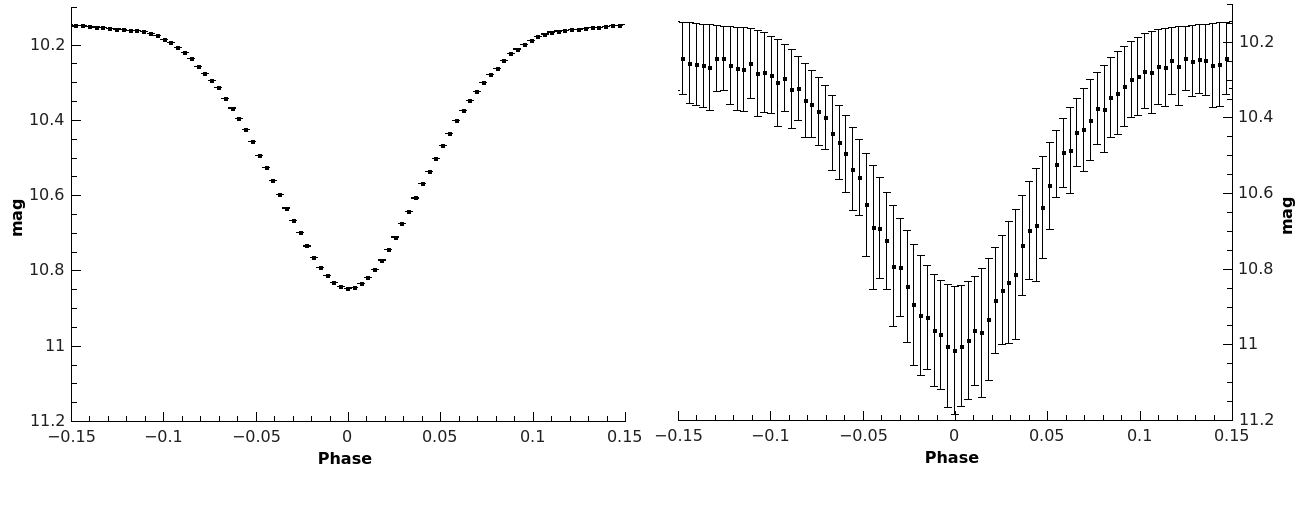
\includegraphics[width=\textwidth]{prec_min//min_err.png}
    \caption{Example of minima with photometry errors 0.0001 mag (left) and 0.1 mag (right)}
    \label{fig:min_err}
\end{figure}

We pick a easiest case -- fitting a classic shape of a minima, and made 1000 simulations of minima determination for both cases. Graphs representing time of minima precision distribution are presented on figure \ref{fig:ph_err_diag}.       

\begin{figure}[!h]
    \centering
    \begin{subfigure}[t]{0.5\textwidth}
        \centering
        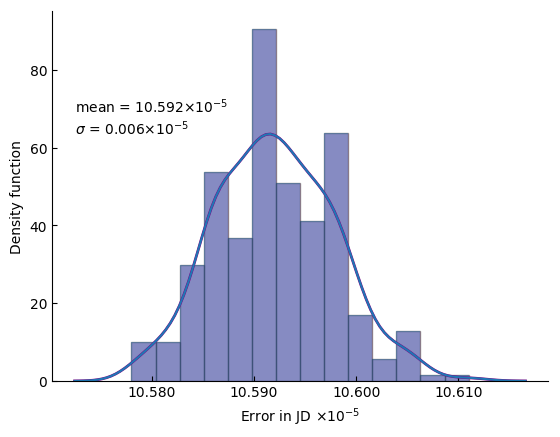
\includegraphics[width=\textwidth]{prec_min//stat_pherr-min.png}
%        \caption{Distribution of errors from LC \\with sampling 20\%}
    \end{subfigure}%
    \begin{subfigure}[t]{0.5\textwidth}
        \centering
        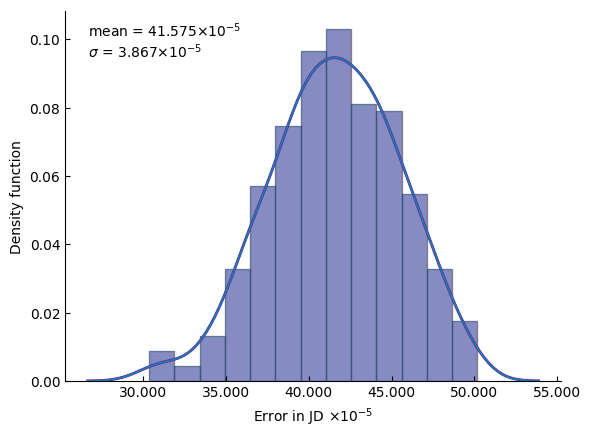
\includegraphics[width=\textwidth]{prec_min//stat_pherr-max.png}
%        \caption{Distribution of errors from LC \\with sampling 80\%}
    \end{subfigure}
    \caption{Distribution of time of minima precision for LC with different photometry accuracy. 0.0001 mag - left, 0.1 mag - right. Blue line is a kernel density estimate.}
\label{fig:ph_err_diag}
\end{figure}
Blue line on figures corresponds to kernel density estimation.
The kernel density estimate (KDE) can be a useful tool for plotting the shape of a distribution. The KDE plots encode the density of observations more clearly then histogram.

As it can be seen from graphs bigger errors (0.1 mag) corresponds to more than two times smaller precision of time of minima determination. Also the standard deviation in case of 0.0001 mag photometry errors is smaller.   

\subsection{Sampling}
According to weather condition, huge errors of photometry, long period of EB system or even some technical issues sampling of data can appear on the light curve.
On next few graphs we will show how sampling affects the precision of minima determination.

As a base we take ideal LC produced by PHOEBE and add the mean photometry error 0.003 mag, which is typical for good weather and telescope with diameter 50 cm with CCD camera. 
We made 1000 simulations of minima determination with random sampling of 20\% of data which is more or less within the bounds of possibility for ground based observations and 1000 simulations of minima determination for 80\% random sampling of data which corresponds to set of bad weather condition or observation of EB system with very long period. 
For example the general look of such LCs are presented on figure \ref{fig:LC_sampl}.

\begin{figure}[!h]
    \centering
    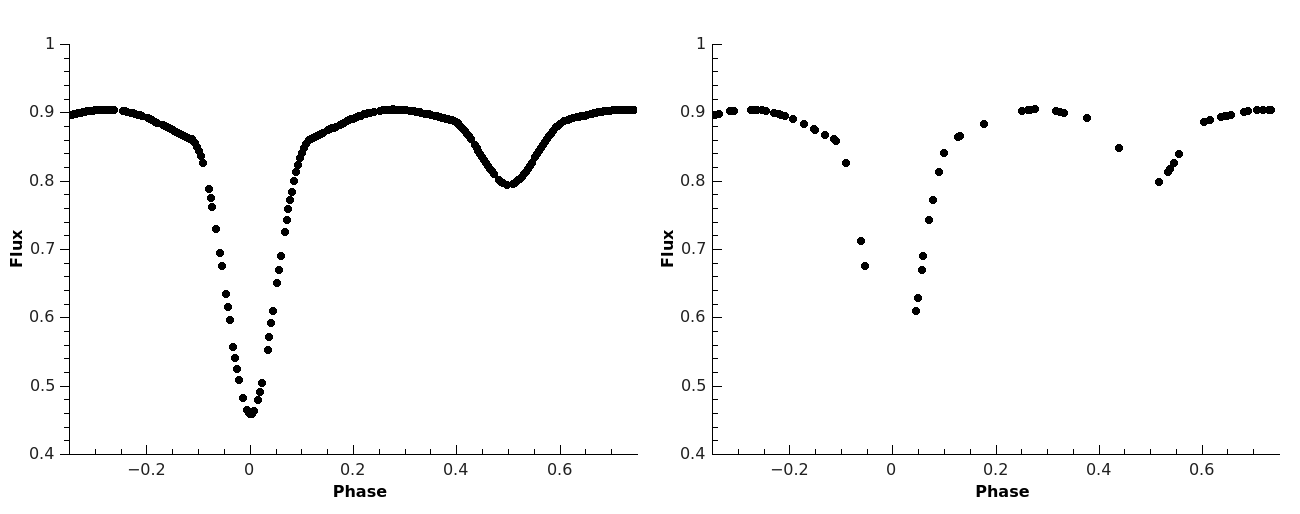
\includegraphics[width=\textwidth]{prec_min//LC_sampl.png}
%    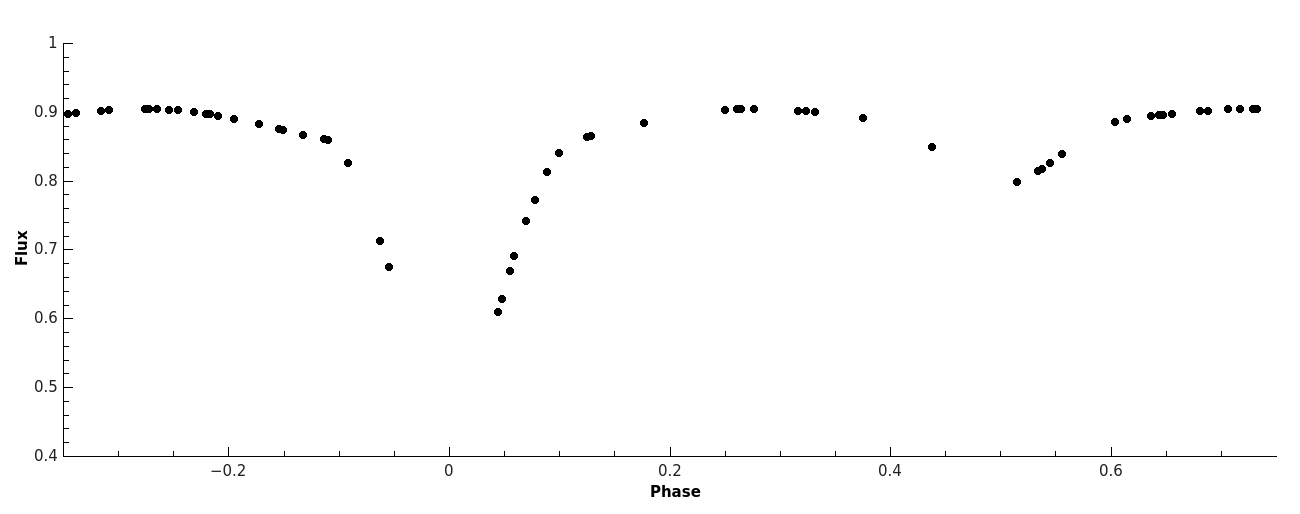
\includegraphics[width=\textwidth]{prec_min//LCs80.png}
    \caption{Example of LC with sampling 20\% (left) and 80\% (right)}
    \label{fig:LC_sampl}
\end{figure}

%\begin{figure}[!h]
%    \centering
%    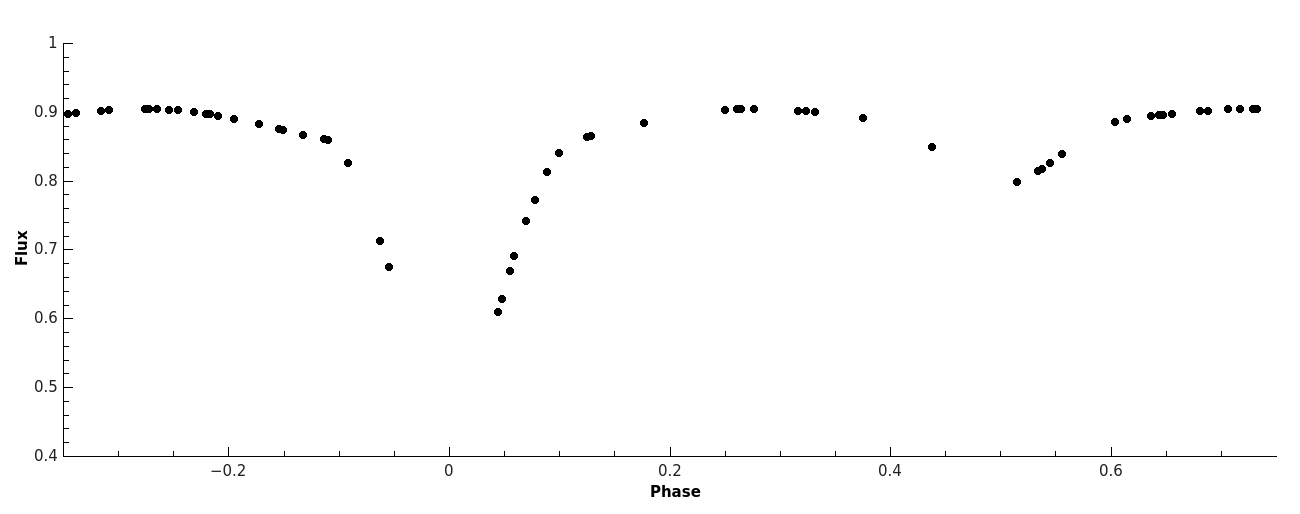
\includegraphics[width=\textwidth]{prec_min//LCs80.png}
%    \caption{LC with sampling 80\%}
%    \label{fig:LC_sampl80}
%\end{figure}

On a figure \ref{fig:sampl_diag} distribution of minima precision is presented for sampling 20\% and 80\%.
Blue line on graph correspond to kernel density estimation.
%The kernel density estimate (KDE) can be a useful tool for plotting the shape of a distribution. The KDE plots encode the density of observations more clearly then histogram.

As it can be expected sampling of data on LC have a great influence on precision of minima determination. 
From Figure \ref{fig:sampl_diag}, we can see that the data with a sampling of 80\% reduces the accuracy of the minimum determination by one order.
%From figure \ref{fig:sampl_diag} we can see that sampling 80\% decrease precision of minima determination in one order.  

\begin{figure}[!h]
    \centering
    \begin{subfigure}[t]{0.5\textwidth}
        \centering
        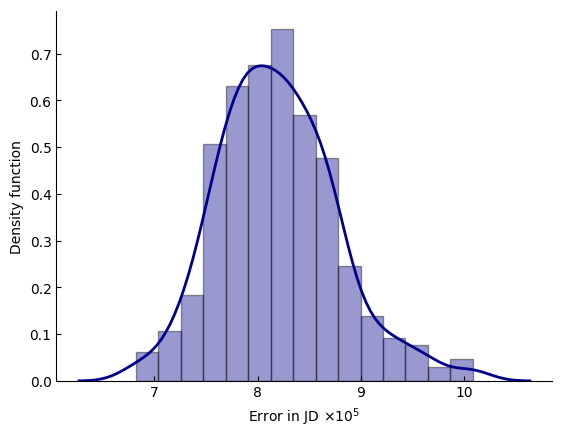
\includegraphics[width=\textwidth]{prec_min//stat-0.2.png}
%        \caption{Distribution of errors from LC \\with sampling 20\%}
    \end{subfigure}%
    \begin{subfigure}[t]{0.5\textwidth}
        \centering
        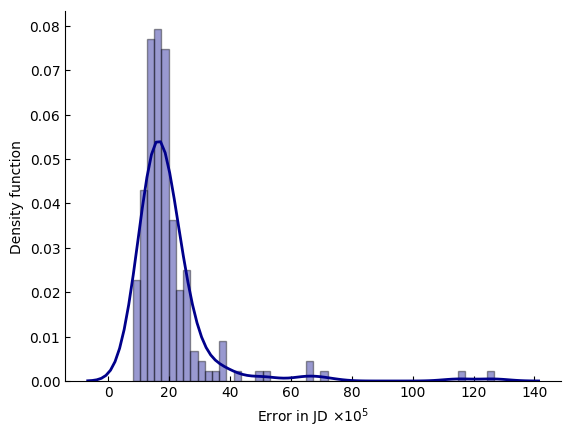
\includegraphics[width=\textwidth]{prec_min//stat-0.8.png}
%        \caption{Distribution of errors from LC \\with sampling 80\%}
    \end{subfigure}
    \caption{Distribution of minima precision from LC with different sampling. 20\% - left, 80\% - right. Blue line is a kernel density estimate.}
\label{fig:sampl_diag}
\end{figure}

%\begin{figure}[!h]
%    \centering
%    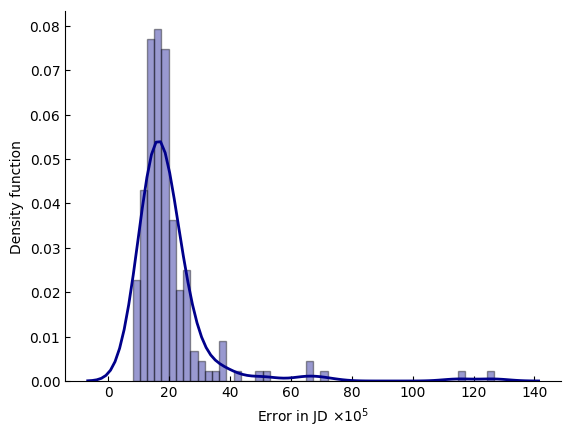
\includegraphics[width=\textwidth]{prec_min//stat-0.8.png}
%    \caption{Distribution of minima precision determinations from LC with sampling 80\%}
%    \label{fig:sampl_diag80}
%\end{figure}
%
%\begin{figure}[!h]
%    \centering
%    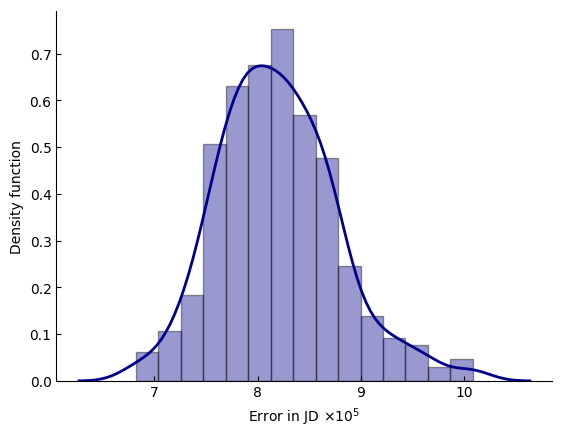
\includegraphics[width=\textwidth]{prec_min//stat-0.2.png}
%    \caption{Distribution of minima precision determinations from LC with sampling 20\%}
%    \label{fig:sampl_diag20}
%\end{figure}

\section{Sampling of data on O-C Diagrams}
5-7 diagrams with different sampling from ideal to few points in different places

\section{Precision of Photometry}
Kepler, Kolonica

\section{Simulations of $3^{rd}$ Body in EB Systems}

In this section, some factors that have an influence on the minima shape, and therefore on O-C diagram too, will be described.  
Such factors are:
\begin{itemize}[noitemsep,nolistsep]
\item EB system visibility from observational point;
\item weather conditions;
\item precision of photometry;
\item presents of spots on EB component, or on both components;
\item pulsation   
\end{itemize}

The O-C diagram of EB system with $3^{rd}$ body would be presented as a ideal conditions case, without any of mentioned above distorting factors, and then compared with conditions close to real one, or under the influence of one of the reviewed factors.

First three factors are not connected with star types, that's why we will consider them separately.
The influence of other factors on O-C diagrams will be considered in the examples of detached and EB contact systems, because of similarity of minima shape in detached, semi-detached and in contact, over-contact EB systems. 

Our simulations are based on a light curves generated by PHOEBE software \citep{Prsa2005} based on well known Wilson \& Devinney code described in work \cite{Wilson1971}. These LC will be extended for needed number of cycles, usually 5 or 10 year. Time shifts in LC caused by presence of $3^{rd}$ body added based on computation made in work \cite{irwin1952, irwin1959}. On the final stage other distortion factors mentioned above are also added to LC.   

\subsection{EB system visibility}

It is good known that periods of star visibility, for some observational point, depend on star declination.
If we proceed from the assumption that observations are collected from one observatory then this feature greatly complicates the task for the observer. In such case there will be only some seasons of observations and gaps in data for a lot of targets. Only near polar regions of sky can be observable throughout the year for middle latitudes observatories.

For example there is two different O-C diagrams presented on Fig. \ref{fig:oc_1}. Left one is for a case when 
target of observation is situated on a equator and right one is for a target near a north pole. Simulations was made for observatory Kolonica AO (Slovakia), duration of observations is 5 years. Parameters of $3^{rd}$ body are presented in second column of table \ref{tab:3rd_body_par}. In a third and fourth columns are orbital parameters obtained by fitting of our O-C diagram with Markov chain Monte Carlo algorithm described in \cite{Gajdos2019}. Same fitting parameters were used for equator and north pole case. We find out that data obtained in the case when the star is situated on the equator are fitted with a worse accuracy and accordingly a star situated near the north pole is fitted better.

\begin{figure}[!h]
    \centering
    \begin{subfigure}[t]{0.5\textwidth}
        \centering
        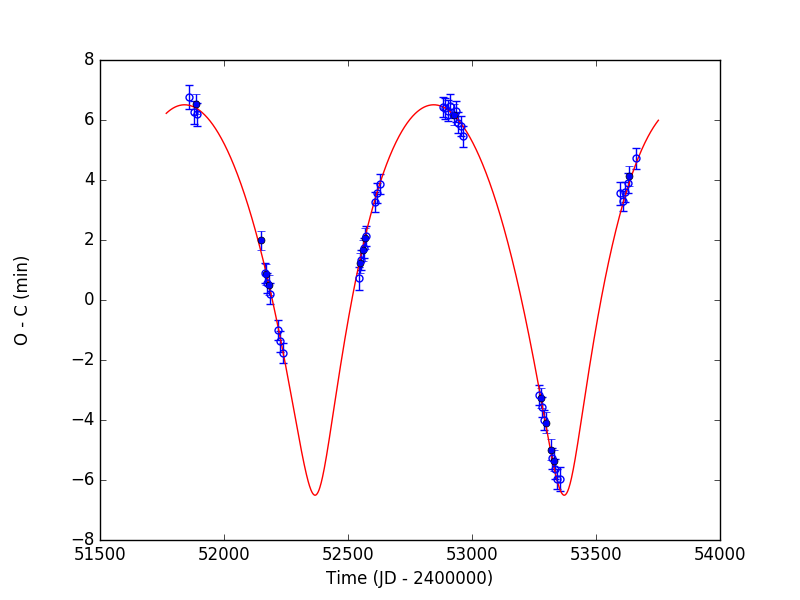
\includegraphics[width=\textwidth]{oc_1_5yrs.png}
        \caption{Star on equator.\\RA = 00:43:45.0838, DEC = +00:00:00}
    \end{subfigure}%
    \begin{subfigure}[t]{0.5\textwidth}
        \centering
        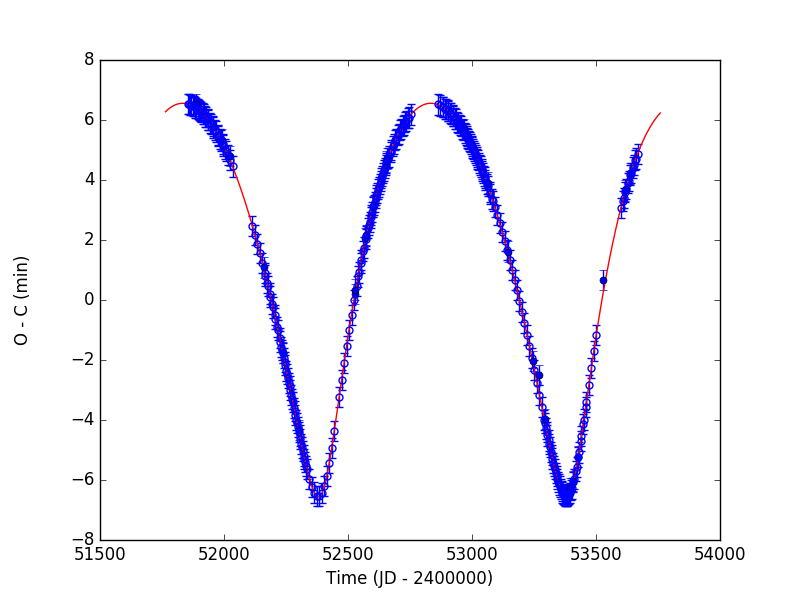
\includegraphics[width=\textwidth]{oc_2_5yrs.png}
        \caption{Star near north pole.\\RA = 00:43:45.0838, DEC = +89:30:00}
    \end{subfigure}
    \caption{O-C diagram for ideal conditions. Red line - fit with MCMC method, correspond to values in table \ref{tab:3rd_body_par}. Filled circles are primary minima, not filled circles - secondary minima. 
    Observatory is Kolonica AO \\(Lat = +48.934917, Lon = 22.2738)}
\label{fig:oc_1}
\end{figure}

\begin{table}[!h]
 \caption{Original parameters of the 3$^{rd}$ body orbit and parameters obtained by fitting $O-C$ diagram simulated in ideal condition on equator and near pole. $P$ -- orbital period of eclipsing pair, $T_0$ -- initial minimum, $P_3$ - orbital period of the 3$^{rd}$ body, $t_{03}$ -- pericenter passage, $a\sin i_3$  -- projected semi-major axis of the orbit, $e_3$ -- eccentricity, $\omega_3$ -- the longitude of the periastron, $f(M_3)$ -- the mass function, $\chi^2$ -- sum of squares of the best fit, $\chi^2/n$ -- reduced sum of squares ($n$ -- number of data points), errors are given in parenthesis.}
 \vspace{-6mm}
 \begin{center}
  \begin{tabular}{lccc}
    \hline
    Solution            & Original                  & Equator               &  near Pole    \\
  \hline\noalign{\smallskip} 
 $P$ [days]             & 1.42834                   & fixed                 & fixed \\ 
 $T_0$ [HJD]            & 2451852.3783              & fixed                 & fixed \\
   \hline\noalign{\smallskip} 
 $P_3$ [days]           &   1000                    & 997(3)                & 999.90(92)\\
 $t_{03}$ [HJD]         & 2451400                   & 2451407(9)            & 2451400(1)    \\
$a\sin i_3$ [AU]        &  0.797                    & 0.807(15)             & 0.8001(35)\\
 $e_3$                  &  0.54                     & 0.55(1)               & 0.5449(45)\\
$\omega_3$ [\degree]    &   288                     & 289(3)                & 288.16(76)\\
\hline\noalign{\smallskip}
$f(M_3)$  [M$_\odot$]   &  --                       & 0.070(4)              & 0.06835(91)\\
\hline\noalign{\smallskip}
$\chi^2$                &  --                       & 8.34                  & 8.323\\
$\chi^2/n$              &  --                       & 0.19                  & 0.026\\
\hline\noalign{\smallskip}
\end{tabular}
\end{center}
\label{tab:3rd_body_par}
\vspace{-6mm}
\end{table}

\subsection{Weather and Photometry Precision}
If we will take into account other factors, like weather and precision of photometry, we will probably get less fit accuracy. 
On the Fig.\ref{fig:oc_weather} (a, b) are presented O-C diagrams with same EB system as in previous case but now we take into account only 45\% of good weather, and photometry precision 0.0001. Such weather condition are rather good for our latitudes, photometry precision 0.0001 can be achieved on 400-600 mm telescopes with modern CCD cameras. Obtained parameters of $3^{rd}$ body orbit are presented in table \ref{tab:3rd_body_w}.

As we can se in table \ref{tab:3rd_body_w}, for a case when star is on equator difference with ideal condition is not so big on $\chi^2/n$ but accuracy of individual parameters is worse. It is because there is not much data point at all for this case.
On the other hand situation for a case when star is near the pole, in comparison with ideal conditions, is getting much worse. 

If we do a simulation of O-C diagrams with more appropriate for our latitudes 30 \% probability of clear sky, values are getting worse. This results are presented on Fig. \ref{fig:oc_weather} (c,d) and in table \ref{tab:3rd_body_w}.

In real life for research of some EB system light curves from many different observatories are used. If this observatories are situated on different latitudes then we will not have such big gaps in our data as can be seen for a case of star on equator. The more observatories contribute to research the less important is influence of weather conditions and object location.
% Weather and photom precision-----------------------------------------
\begin{figure}[!h]
    \centering
    \begin{subfigure}[t]{0.5\textwidth}
        \centering
        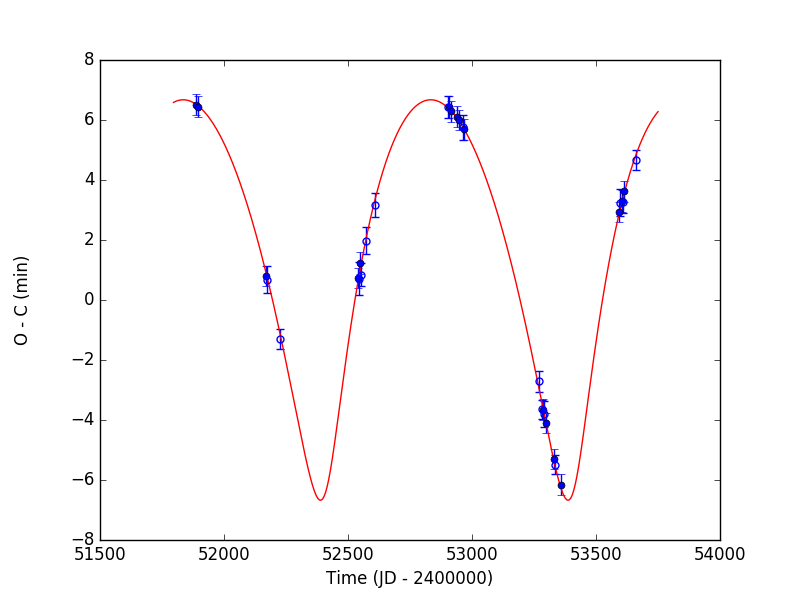
\includegraphics[width=\textwidth]{oc_w.png}
        \caption{Star on equator. 45\% of clear nights.\\RA = 00:43:45.0838, DEC = +00:00:00}
    \end{subfigure}%
    \begin{subfigure}[t]{0.5\textwidth}
        \centering
        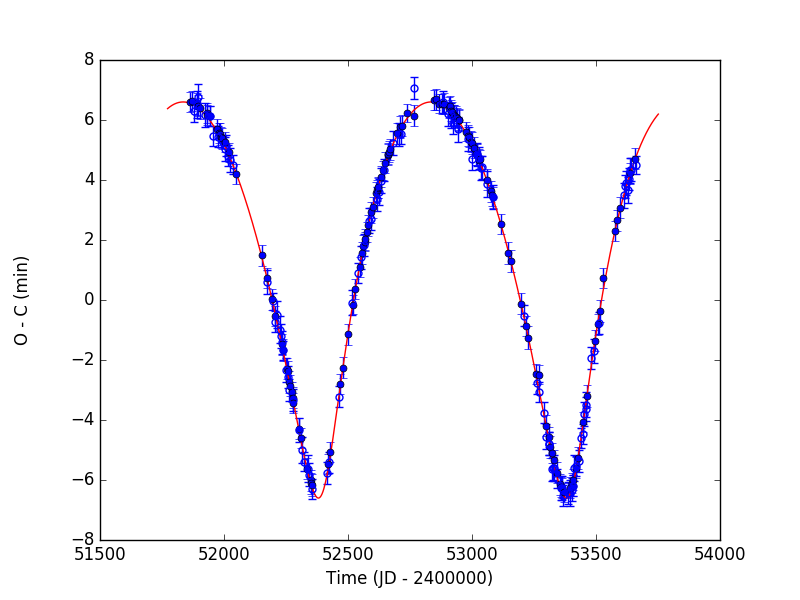
\includegraphics[width=\textwidth]{oc_eq_w2.png}
        \caption{Star near north pole. 45\% of clear nights\\RA = 00:43:45.0838, DEC = +89:30:00}
    \end{subfigure}
    
    \begin{subfigure}[t]{0.5\textwidth}
        \centering
        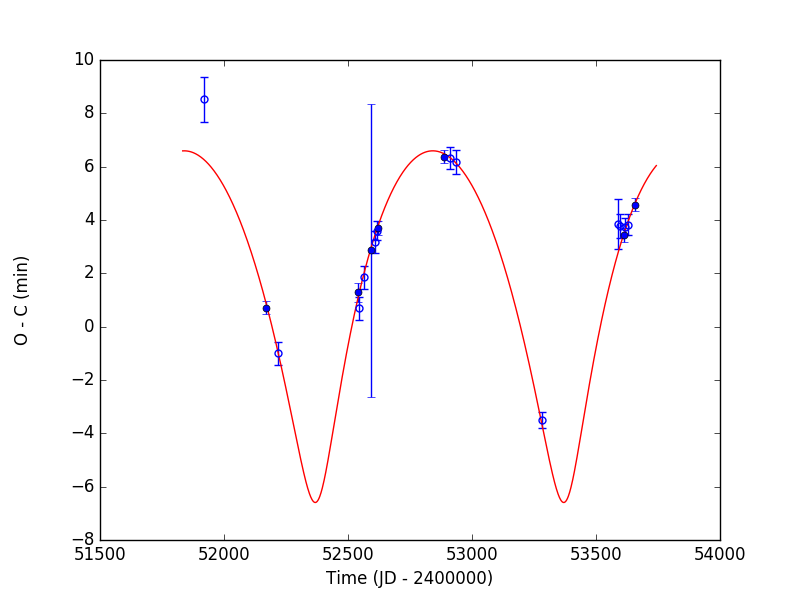
\includegraphics[width=\textwidth]{oc_w30_e.png}
        \caption{Star on equator. 30\% of clear nights\\RA = 00:43:45.0838, DEC = +00:00:00}
    \end{subfigure}%
    \begin{subfigure}[t]{0.5\textwidth}
        \centering
        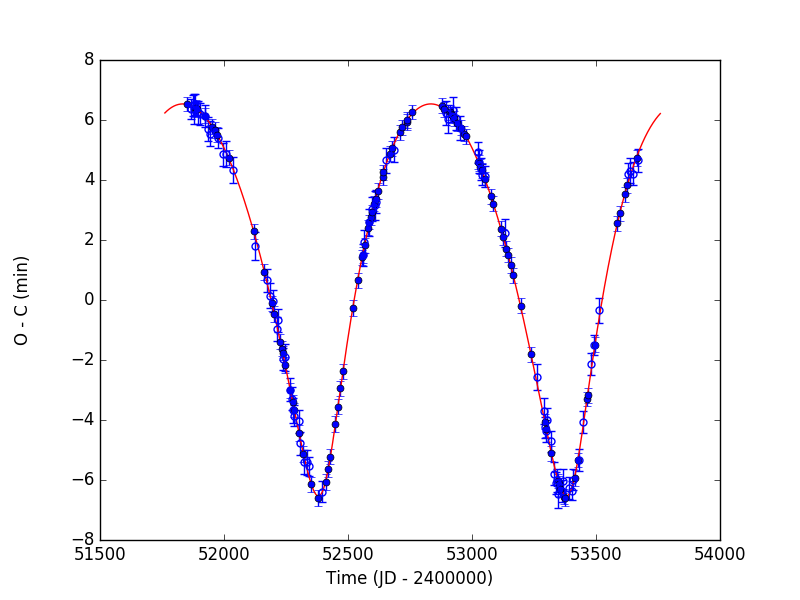
\includegraphics[width=\textwidth]{oc_w30_p.png}
        \caption{Star near north pole. 30\% of clear nights\\RA = 00:43:45.0838, DEC = +89:30:00}
    \end{subfigure}
    \caption{O-C diagram for 45\% (a,b) and 30\% (c,d) of good weather and photometry accuracy 0.0001.
    Red line - fit with MCMC method, correspond to values in table \ref{tab:3rd_body_w}. Filled circles are primary minima, not filled circles - secondary minima. Observatory is Kolonica AO \\(Lat = +48.934917, Lon = 22.2738)}
\label{fig:oc_weather}
\end{figure}


\begin{table}[!h]
 \caption{Original parameters of the 3$^{rd}$ body orbit and parameters obtained by fitting $O-C$ diagram simulated with influence of weather (45\% and 30\% of clear nights) and photometry precision 0.0001. For description of parameters see Table \ref{tab:3rd_body_par}}
 \vspace{-6mm}
 \begin{center}
  \begin{tabular}{lccccc}
    \hline
    Solution            & Original                  & Equator 45 \%         &  Pole 45\%          & Equator 30\%  &  Pole 30\%        \\
  \hline\noalign{\smallskip}                                                                                                                 
 $P$ [days]             & 1.42834                   & fixed                 & fixed               & fixed        & fixed             \\ 
 $T_0$ [HJD]            & 2451852.3783              & fixed                 & fixed               & fixed        & fixed             \\
   \hline\noalign{\smallskip}                                                                                                         
 $P_3$ [days]           &   1000                    & 998(4)                & 1000(1)             & 1002(5)      & 999(1)            \\
 $t_{03}$ [HJD]         & 2451400                   & 2451413(11)           & 2451398(3)          & 2451376(16)  & 2451399(3)       \\
$a\sin i_3$ [AU]        &  0.797                    & 0.819(22)             & 0.805(4)            & 0.797(22)    & 0.801(5)          \\
 $e_3$                  &  0.54                     & 0.553(14)             & 0.5588(57)          & 0.569(23)    & 0.558(6)        \\
$\omega_3$ [\degree]    &   288                     & 291(5)                & 287.6(9)            & 280(5)       & 289(1)          \\
\hline\noalign{\smallskip}                                                                                                                   
$f(M_3)$  [M$_\odot$]   &  --                       & 0.074(6)              & 0.069(1)            & 0.067(6)     & 0.069(1)          \\
\hline\noalign{\smallskip}                                                                                                               
$\chi^2$                &  --                       & 4.82                  & 36.46               & 15.00        & 31.29              \\
$\chi^2/n$              &  --                       & 0.18                  & 0.16                & 1.00         & 0.18              \\
\hline\noalign{\smallskip}

\end{tabular}
\end{center}
\label{tab:3rd_body_w}
\vspace{-6mm}
\end{table}

\subsection{Spots in EB Systems}
In previous subsections, we were dealing with terrestrial factors that cause inaccuracy in O-C diagrams. 
Now we will try to simulate O-C diagrams in ideal terrestrial conditions but under the influence of other non-terrestrial factors like starspots.

As we know the formation of starspots depends on the age of a host star, that's why we should separate our simulation on detached and contact EB systems. 
But before we start to simulate we need to know some general spot parameters for this EB systems. Its a radius of star spot, its temperature, and life cycle. Do the spot disappear after some short time or can be present on a host star for a relatively long time like 5-10 years? The spots migrate or not?  

In work \cite{Kalimeris2002} authors have
shown that intensity variations resulting from star-spots (not taking into account Wilson depressions) can introduce disturbances of
up to $\sim 0.01$~day in the O-C residuals of contact binaries. Given the
rapid evolutionary time-scales of spots (of the order of days) seen in
recent Doppler images of the contact binary AE Phe \citep{Barnes2004} 
this may lead to explaining some of the observed jitter in the
O-C curves of these objects. But in work \cite{Watson2004}, the effects of a
Wilson depression seem to result in a scatter of only a few seconds
in the O-C residuals, it seems unlikely that the Wilson depression
will be a significant source of jitter for contact binaries.
Such changes resulting from star-spots
would be distinguishable from other mechanisms that cause period
changes and it should still be possible to determine the orbital period accurately  \citep{Watson2004}.

Several studies have indicated that spot on close binaries can have angular diameters from $10\degree$ to $40\degree$ which means that they
will cover from 5 to 25\% of the whole photosphere of the active components (e.g. \cite{Hall1990, Guinan1993}).
In most cases, active component can have one or two giant spots. It is also argued that such spots can remain on a surface from a few years to even ten years \citep{Kalimeris2002}. 

For a estimation of maximum effect caused by the star spot, it is assumed that in our simulations spots are located on equator of each component.
According to \cite{Kalimeris2002} spots with angular diameter less then $10\degree$ cause negligible shifts of the light minimum of the primary eclipse. Therefore we will not consider with spots smaller then $10\degree$ (see fig. \ref{fig:spot_diam}).

Furthermore, the spots on secondary component always remain visible during the primary eclipse,
while the spots on primary do not. As a result, the spots on primary cause a
significantly greater photometric perturbation to the light curve than the spots on secondary component.

\citeauthor{Kalimeris2002} also showed that unlike real orbital period changes, non-migrating star spots cannot
cause permanent slopes in the O-C diagrams. 
But the O-C differences caused by long-lived migrating spots can be expected to be periodic.

\begin{figure}[!h]
\vspace{0cm}
\centerline{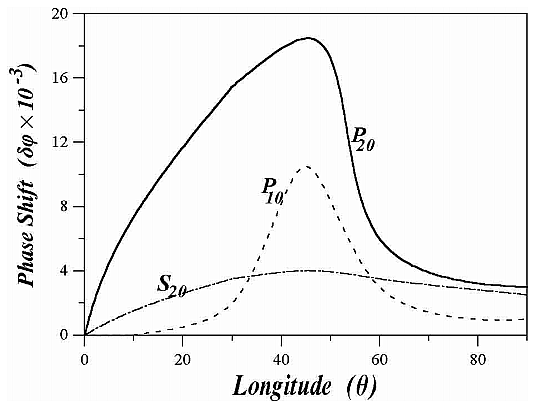
\includegraphics[width=0.60\textwidth]{spot_diam_2.png}}
\caption{Phase shift $\delta\varphi(\theta)$ of the primary eclipse of a contact
binary similar to AB And. Curves labelled by "P" correspond
to a spot on the primary, while "S" refers to a spot on the
secondary component. \citep{Kalimeris2002}.}
\label{fig:spot_diam}
\end{figure}   
 

\subsubsection{Detached EB Systems}
% Pro single stars
%Younger stars rotate faster than older stars and
%have higher activity levels and greater spot coverage (????). As a result, there is an overall trend of the
%degree of photometric variability with age. % \cite article "The Ages of Stars".

Tidal interactions force most of these stars to rotate synchronously with their orbital motions.
The rapid rotation combined with deep convection envelopes produces a variety of magnetic activity phenomena including starspots in these stars.

Brightness variations due to starspots can be observed in detached EB only during primary total eclipses when the luminous hot components are hidden. Therefore, because of synchronized rotation, only one hemisphere of the cool stars can be observed and the photometric data collected are less detailed than for other spotted binaries \citep{Berdyugina2005}.
 
For detached eclipsing binary systems spots with radius from 5\degree~to~25\degree are usually typical, we can find such systems in many publications like e.g. \cite{Liakos2011} or in publications about spots in RSCVn binaries systems (e.g. \cite{Roettenbacher2011, Kovari2012, Kozhevnikova2015}). Objects with spots migrations are very rarely observed, so we will not consider such a case.
Model of detached EB system is presented on figure \ref{fig:eb_det_model}, the main parameters of this system are listed in the table \ref{tab:detached_params}.

As we mentioned above, spots with a radius less then 10\degree~ do not have a big influence on O-C diagram. So, we will consider how starspot located on stars equator (colat=90\degree, lon=0\degree) with radius $r_{spot}=15\degree$ and $r_{spot}=25\degree$~ affect the O-C diagram. 
There is also a difference in a hot and cold spot. The hot spot will have $T_{spot}=1.2$, where $T_{spot}$ is the ratio between the temperature of the spot and the local temperature of the underlying photosphere, the cold spot will be defined as $T_{spot}=0.8$. On figure \ref{fig:detached_spots} we can see how hot and cold spots affect the shape of the minima. Mainly primary minima are changing their shape under the influence of spots.

\begin{figure}[!h]
\vspace{0cm}
\centerline{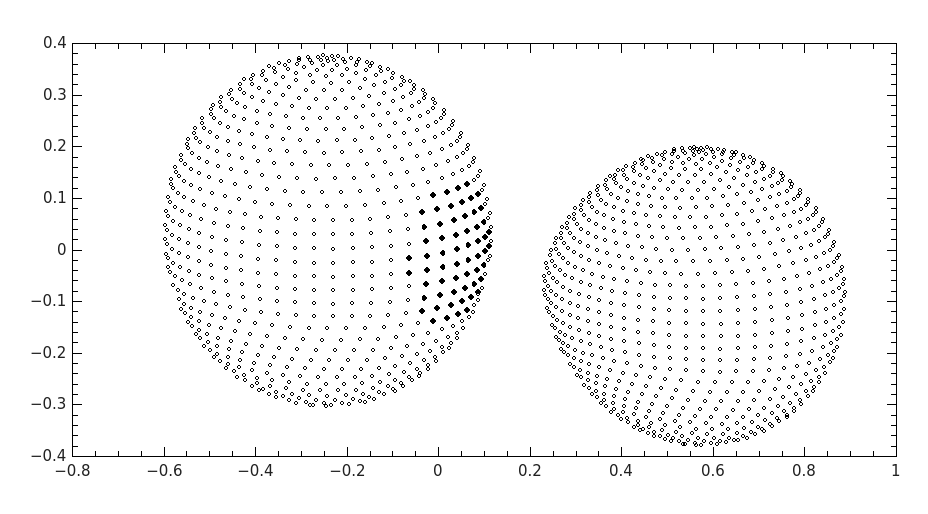
\includegraphics[width=0.80\textwidth]{detached_pspot_08-25_view.png}}
\caption{Model of detached EB system with spot (colat=90\degree, colon=0\degree) in plane of sky view at phase 0.15.}
\label{fig:eb_det_model}
\end{figure}

\begin{table}[!h]
 \caption{Basic parameters of detached binary system presented on figure~ \ref{fig:eb_det_model}. HJD0 is a origin of the
 ephemeris; P - orbital period of EB system; SMA - semi-major axis; RM - mass ratio; VGA - centre of mass velocity, \\INCL - inclination}
 \begin{center}
 \vspace{-6mm}
  \begin{tabular}{c|c}
    \hline 
HJD0(day) & 2451852.3783\\
P(day)    & 1.42834\\
\hline
SMA ($R_\odot$) &  1.000\\
RM              &  0.432\\
VGA (km/s)      &  0\\
INCL (\degree)  & 77.690\\
\hline
\end{tabular}
\end{center}
\label{tab:detached_params}
\vspace{-6mm}
\end{table}

\begin{figure}[!h]
    \centering
    \begin{subfigure}[t]{0.5\textwidth}
        \centering
        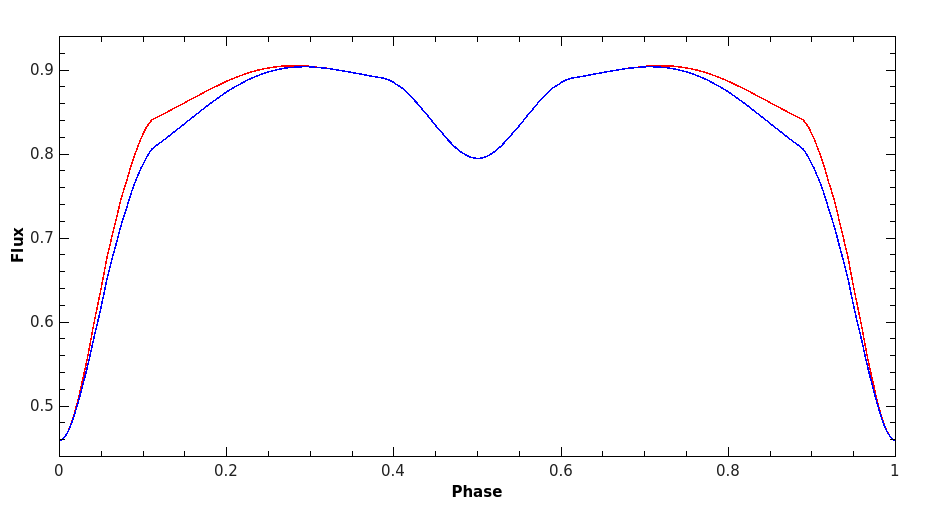
\includegraphics[width=\textwidth]{detached_pspot_08.png}
        \caption{Spot with $T_{spot}=0.8$}
    \end{subfigure}%
    \begin{subfigure}[t]{0.5\textwidth}
        \centering
        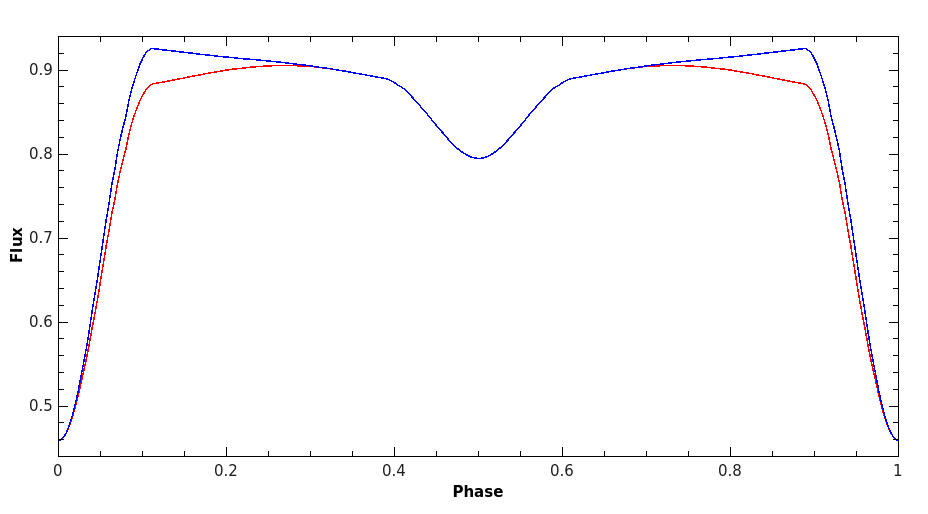
\includegraphics[width=\textwidth]{detached_pspot_12.png}
        \caption{Spot with $T_{spot}=1.2$}
    \end{subfigure}
    \caption{Spot on primary component with different temperature and radius. 
    Blue line - spot radius 25\degree, red line - spot radius 15\degree}
\label{fig:detached_spots}
\end{figure}

The final O-C diagrams for all four cases are presented in figure \ref{fig:oc_detached_spot}. Looking only on O-C diagram we can't clearly see the difference. Only when we fit these O-C diagrams by MCMC method results are getting clearer. 
Final solutions of fitting are presented in table \ref{tab:3rd_body_detached_spot}. Analysing $\chi^2$ value of 4 cases we can state that 
case of spot with parameters $T_{spot}=1.2$ and $r_{spot}=25\degree$ is fitted the best. The precision of fit depends on the accuracy of minima determination that can vary depending on the method we used. In case of a spot with parameters $T_{spot}=1.2$ and $r_{spot}=25\degree$ precision of minima determination was almost the same for primary and secondary minima. 

%are almost the same, except case of spot with $T_{spot}=1.2$ and $r_{spot}=25\degree$, in this case $\chi^2$ is the best. 
%But if we take into account Bayesian information criterion (BIC) and Akaike information criterion (AIC), where bigger value corresponds to better fit, the situation changes to the opposite. 
%Best fit is case with small cold spot, and worst fit is case with hot and big spot.\\
%(RECALCULATE!!!!!) 

\begin{figure}[!h]
    \centering
    \begin{subfigure}[t]{0.5\textwidth}
        \centering
        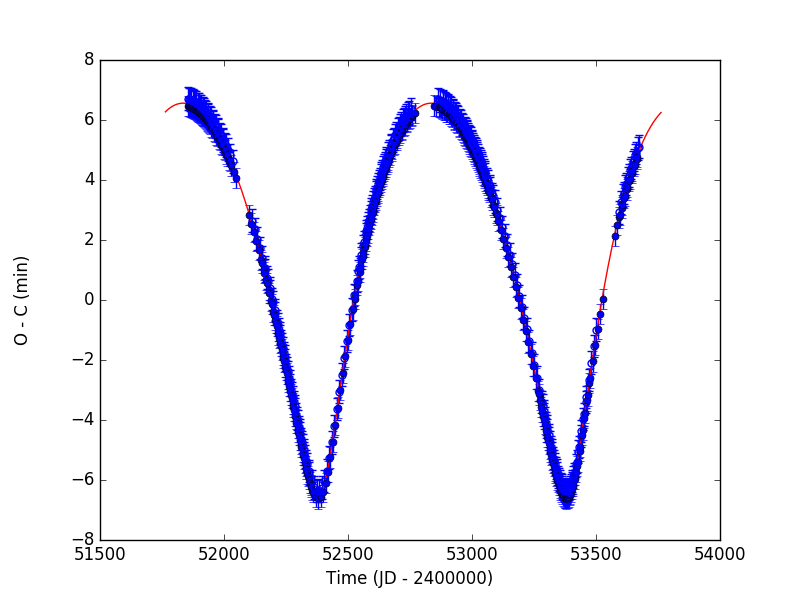
\includegraphics[width=\textwidth]{oc_detached_pspot_R15_T12.png}
        \caption{O-C diagram with $r_{spot}=15, T_{spot}=1.2$}
    \end{subfigure}%
    \begin{subfigure}[t]{0.5\textwidth}
        \centering
        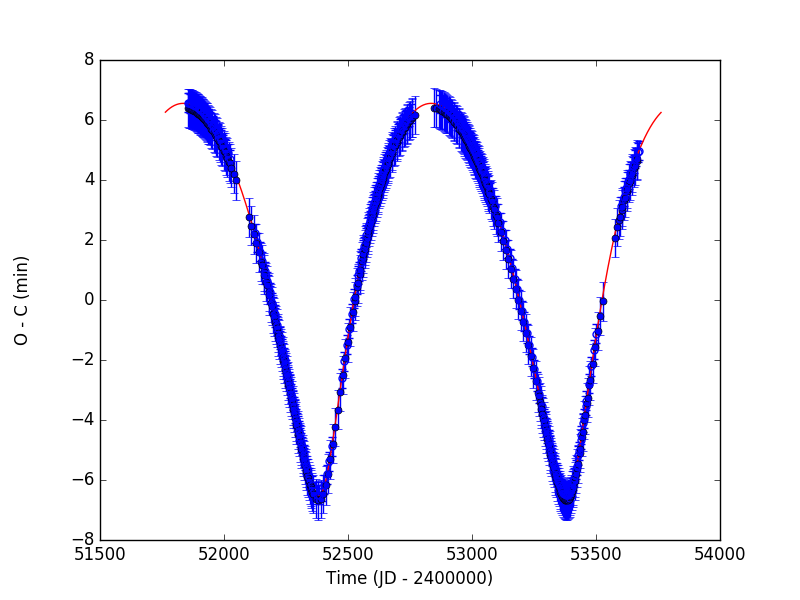
\includegraphics[width=\textwidth]{oc_detached_pspot_R25_T12.png}
        \caption{O-C diagram with $r_{spot}=25, T_{spot}=1.2$}
    \end{subfigure}
    
    \begin{subfigure}[t]{0.5\textwidth}
        \centering
        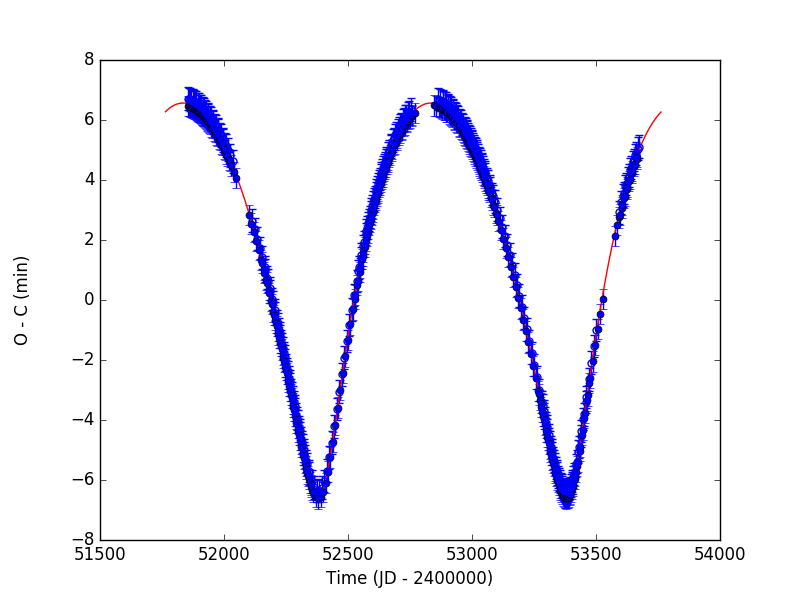
\includegraphics[width=\textwidth]{oc_detached_pspot_R15_T08.png}
        \caption{O-C diagram with $r_{spot}=15, T_{spot}=0.8$}
    \end{subfigure}%
    \begin{subfigure}[t]{0.5\textwidth}
        \centering
        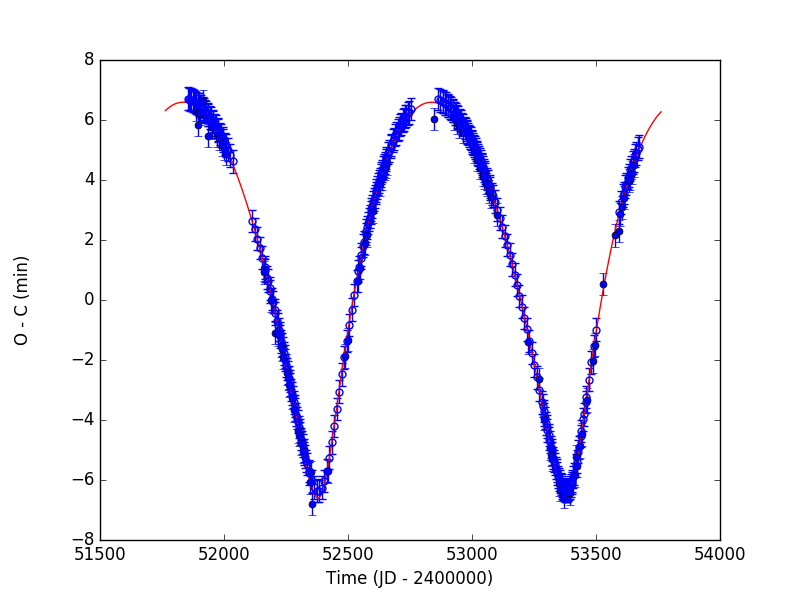
\includegraphics[width=\textwidth]{oc_detached_pspot_R25_T08.png}
        \caption{O-C diagram with $r_{spot}=25, T_{spot}=0.8$}
    \end{subfigure}
    \caption{O-C diagram for EB system with different $r_{spot}$ and $T_{spot}$\\
    Red line - fit with MCMC method, correspond to values in table \ref{tab:3rd_body_detached_spot}. 
    Filled circles are primary minima, not filled circles - secondary minima.}
\label{fig:oc_detached_spot}
\end{figure}


\begin{table}[!h]
 \caption{Orbital parameters of $3^{rd}$ body for detached EB system with different spot parameters $r_{spot}$ and $T_{spot}$. 
 For description of parameters see Table~\ref{tab:3rd_body_par}}
  \vspace{-6mm}
 \begin{center}
  \begin{tabular}{lccccc}
    \hline
    Solution            & Original       & $r_{spot}$=25\degree&$r_{spot}$=25\degree  &$r_{spot}$=15\degree &$r_{spot}$=15\degree \\
                        &                &    $T_{spot}$=1.2    &  $T_{spot}$=0.8 &  $T_{spot}$=1.2  &  $T_{spot}$=0.8 \\
  \hline\noalign{\smallskip}                                                                                                                 
 $P$ [days]             & 1.42834        &           fixed     & fixed       & fixed        & fixed       \\ 
 $T_0$ [HJD]            & 2451852.3783   &           fixed     & fixed       & fixed        & fixed       \\
   \hline\noalign{\smallskip} 
% $P_3$ [days]           &   1000         &          999.9(9)   & 1001(1)     &   1000.7(9)  &  999.8(7)   \\       
% $t_{03}$ [HJD]         & 2451400        &          2451400(2) & 2451394(2)  &   2451397(2) &  2451400(1) \\
%$a\sin i_3$ [AU]        &  0.797         &          0.799(3)   & 0.803(3)    &   0.799(3)   &  0.801(2)   \\     
% $e_3$                  &  0.54          &          0.541(4)   & 0.566(5)    &   0.548(3)   &  0.547(3)   \\            
%$\omega_3$ [\degree]    &   288          &          287.8(7)   & 286.6(8)    &   287.4(8)   &  288.0(5)   \\     
%\hline\noalign{\smallskip}                                                                                                 
%$f(M_3)$  [M$_\odot$]   &  --            &          0.0681(8)  & 0.0689(9)   &   0.0681(7)   &  0.0686(7)  \\       
%\hline\noalign{\smallskip}                                                                                             
%$\chi^2$                &  --            &          21.714     & 54.867      &  74.652      &  74.168     \\        
%$\chi^2/n$              &  --            &           0.0347    & 0.1432      &   0.1161     &   0.1153    \\ 
                                                                                                        
 $P_3$ [days]           &   1000         &          1000(1)    & 1000.0(7)   &   1000(1)    &  1000.8(9)   \\       
 $t_{03}$ [HJD]         & 2451400        &          2451397(3) & 2451397(1)  &   2451396(2) &  2451396(2) \\
$a\sin i_3$ [AU]        &  0.797         &          0.801(2)   & 0.803(3)    &   0.806(4)   &  0.802(3)   \\     
 $e_3$                  &  0.54          &          0.552(3)   & 0.559(4)    &   0.572(5)   &  0.563(3)   \\            
$\omega_3$ [\degree]    &   288          &          287.2(8)   & 287.1(6)    &   286.9(8)   &  286.9(7)   \\     
\hline\noalign{\smallskip}                                                                                                 
$f(M_3)$  [M$_\odot$]   &  --            &          0.0685(7)  & 0.0690(7)   &   0.0697(10) &  0.0691(7)  \\       
\hline\noalign{\smallskip}                                                                                             
$\chi^2$                &  --            &          7.326      & 35.990      &  30.227      &  39.209     \\        
$\chi^2/n$              &  --            &           0.0127    & 0.0654      &   0.0767     &   0.0993    \\       
% AIC                    &  --            &          31.714     & 64.867      &  84.652      &  84.168     \\
% BIC                    &  --            &          53.942     & 84.672      & 107.022      & 106.538     \\
\hline\noalign{\smallskip}  

\end{tabular}
\end{center}
\label{tab:3rd_body_detached_spot}
\vspace{-6mm}
\end{table}

It was mentioned above that spot on secondary component do not have a big influence on minima shape, so we will not consider here this option.

As a conclusion we can say that detached EB systems with spot are not sophisticated objects for $3^{rd}$ body detection. In case of bigger then 25\degree ~spots on the surface it is advisable to cut off from the top the height of primary (or secondary) minima to get better fit and to determine the time of minima more precisely.
 
\subsubsection{Contact EB Systems}
Contact binary stars occur relatively often among binaries (95\% of eclipsing binary
variables in the solar neighbourhood) \cite{Rucinski98}. 
A contact binary system consists of two dwarf stars, most often from the F, G, and K
spectral classes, that are surrounded by a common convective envelope. 
The orbital period distribution peaks in the 8 to 12 hour range. Most systems, though not all,
have orbital periods between 0.2 and 1.0 days \citep{Maceroni96, Paczynski2006}. 
While the masses of the two component stars of a contact binary
are typically unequal, the two stars usually have approximately equal surface temperatures due to the effects of
mass and energy transfer between the components via a common convective envelope \citep{Lucy68}. 
Eclipsing contact binaries are often referred to as W UMa systems in honor of the prototype \citep{Tran2013}.

The components of such a contact binary rotate very rapidly in spite of their old ages
($v~sin~i \sim 100 - 200~ km~s^{-1}$ ) as a result of spin-orbit synchronisation due to strong tidal interactions between the stars \citep{Berdyugina2005}. 

%Observations reveal that there are two subclasses of W UMa stars: A-type and W-type systems.
%The former have longer periods, are hotter, have larger total mass, and a smaller mass-ratio and
%are in better contact.
Many contact binaries show signs of stellar activity, presumably because the component stars are rapid
rotators with deep convective zones. 
A study of the contact binaries with Doppler imaging
technique reveals that both components can be covered by cool starspots, with
a tendency for the primary to be more active than the secondary \citep{Maceroni94, Hendry2000, Barnes2004}.

This makes contact binaries excellent laboratories in
which to investigate the temporal variations and evolution of stellar spots, in part because the timescales of
the variations are shorter than in other types of binary and single stars. 
However, the shortest among these timescales can be problematic to study using groundbased observatories because they are comparable to the
length of an Earth night.

\begin{figure}[!h]
\vspace{0cm}
\centerline{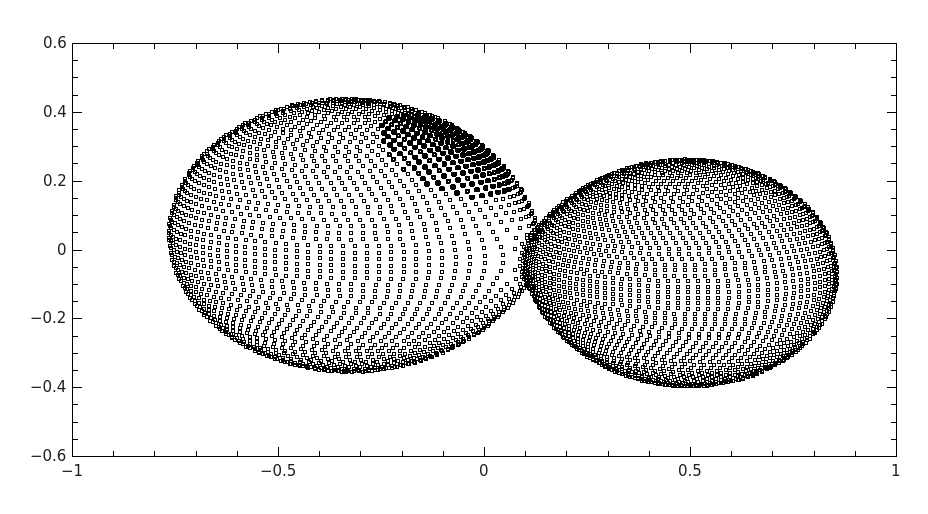
\includegraphics[width=0.8\textwidth]{Overcontact_mesh.png}}
\caption{Model of contact EB system with spot (colat=45\degree, colon=0\degree) in plane of sky view at phase 0.15.}
\label{fig:eb_overcont_model}
\end{figure}


\begin{table}[!h]
 \caption{Baisic parameters of contact binary system presented on figure~ \ref{fig:eb_overcont_model}. HJD0 is a origin of the
 ephemeris; P - orbital period of EB system; SMA - semi-major axis; RM - mass ratio; VGA - centre of mass velocity, \\INCL - inclination}
 \begin{center}
 \vspace{-6mm}
  \begin{tabular}{c|c}
    \hline 
HJD0(day) & 2451852.3783\\
P(day)    & 1.42834\\
\hline
SMA ($R_\odot$) &  1.76\\
RM              &  0.67\\
VGA (km/s)      &  4.70\\
INCL (\degree)  & 79.50\\
\hline
\end{tabular}
\end{center}
\label{tab:overcontact_params}
\vspace{-6mm}
\end{table}

\cite{Kalimeris2002} noted that the migration of
starspots on the surface(s) of the constituent stars in
short-period binaries, especially contact binaries, could
affect measurements of eclipse times and thereby mimic
changes in the orbital period \citep{Tran2013}. 
%\cite{Kalimeris2002} also
%showed that the perturbations to the O-C diagrams would generally have amplitudes smaller than $\sim 0.01$ days, and could appear to
%be quasiperiodic on timescales of a few hundred days or so if the spot migration is related to differential rotation
%of the host star \citep{Tran2013}.

Model of contact EB system with spot is presented on figure \ref{fig:eb_overcont_model}, orbital parameters can be found in table \ref{tab:overcontact_params}. 

\begin{figure}[!h]
    \centering
    \begin{subfigure}[t]{0.5\textwidth}
        \centering
        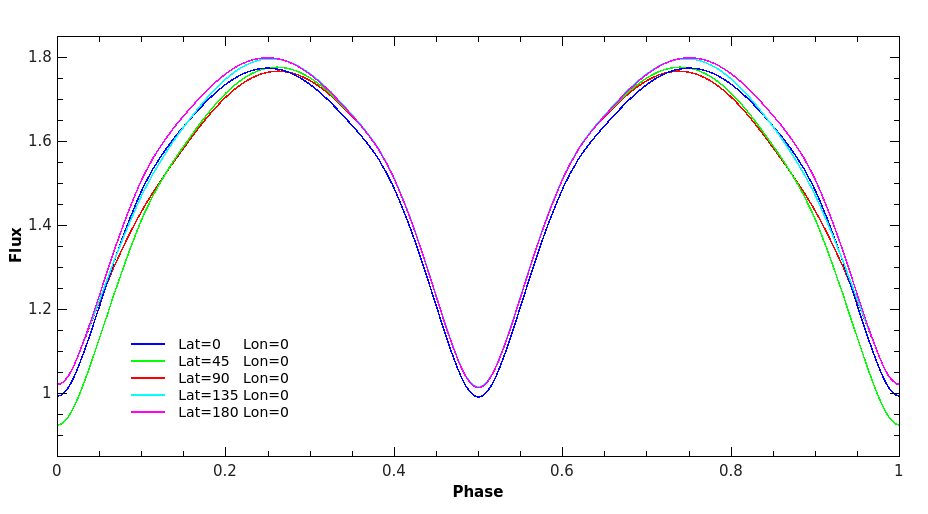
\includegraphics[width=\textwidth]{Overc_spot_pos_lat.png}
        \caption{LC with spot on different colatitude and \\longitude = 0\degree}
    \end{subfigure}%
    \begin{subfigure}[t]{0.5\textwidth}
        \centering
        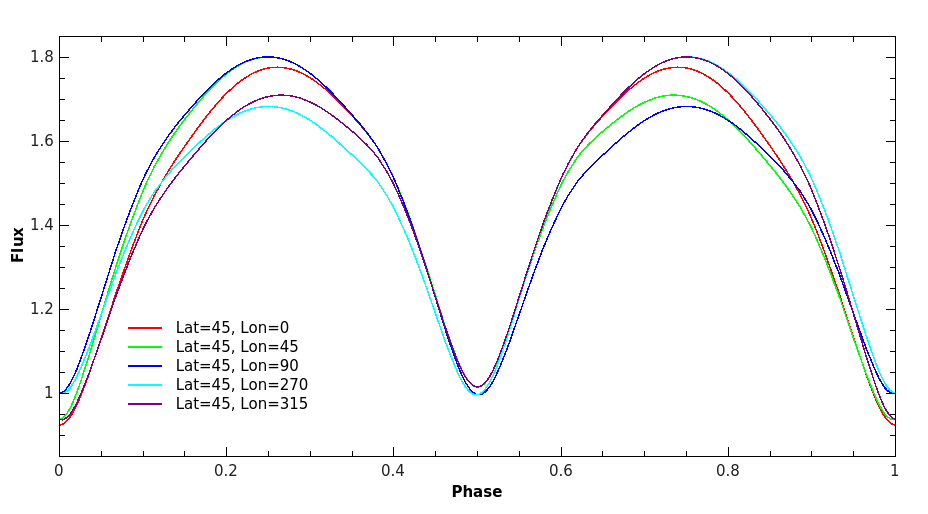
\includegraphics[width=\textwidth]{Overc_spot_pos_lon.png}
        \caption{LC with spot on different longitude and \\colatitude = 45\degree}
    \end{subfigure}
    \caption{LC of contact binary system with "cold" spot ($T_{spot}=0.8~T_{surf}$) on primary component at different positions}
\label{fig:overcontact_spot_pos}
\end{figure}

Light curve from such EB system will be subjected to changes depending on the position of the spot, such changes are partially presented on figure \ref{fig:overcontact_spot_pos}, \ref{fig:overcontact_spotT12_pos}. Analyzing these data we can conclude that the most noticeable changes in LC are caused by changes of position in longitude of a starspot on the primary component of contact binary EB system.
If we change spot position only in colatitude and leave longitude equal to 0\degree, we will observe only variation of primary minima shape and depth. On the other hand if we make colatitude constant (colatitude = 45\degree~ on figures \ref{fig:overcontact_spot_pos}, \ref{fig:overcontact_spotT12_pos}) and change longitude of spot then in addition to the primary minimum part of the LC between two minima will vary too. As it can be expected "hot" spot has a greater contribution to changes in LC than "cold" spot (see fig \ref{fig:overcontact_spot_pos}b vs \ref{fig:overcontact_spotT12_pos}b). 

\begin{figure}[!h]
    \centering
    \begin{subfigure}[t]{0.5\textwidth}
        \centering
        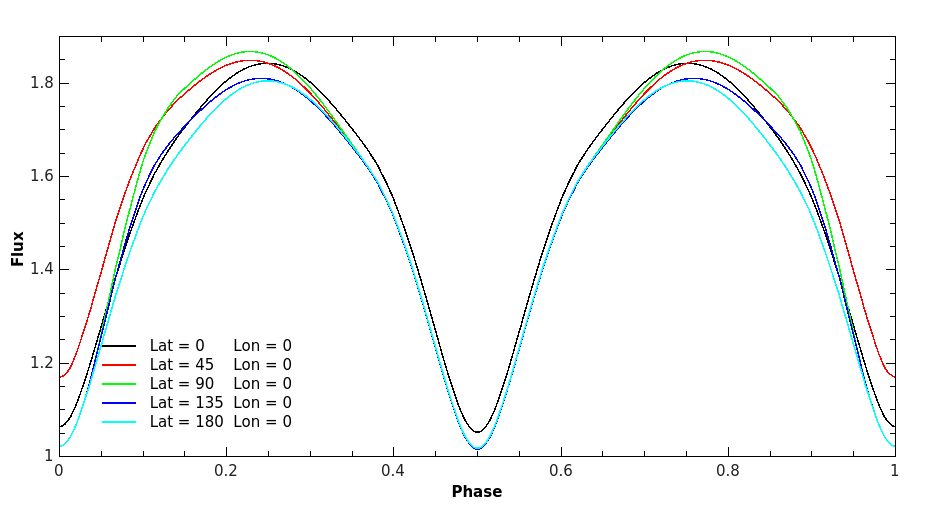
\includegraphics[width=\textwidth]{overc_spotT12_pos_lat.png}
        \caption{LC with spot on different colatitude and \\longitude = 0\degree}
    \end{subfigure}%
    \begin{subfigure}[t]{0.5\textwidth}
        \centering
        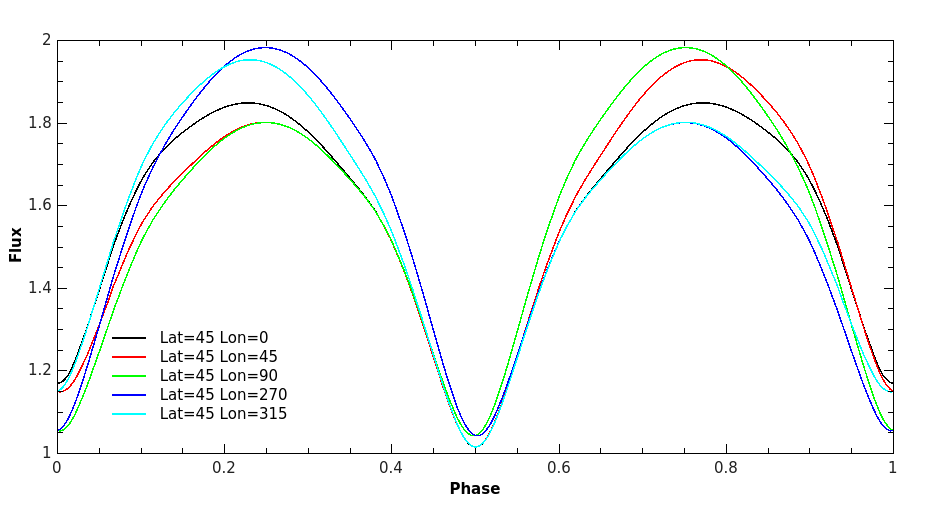
\includegraphics[width=\textwidth]{overc_spotT12_pos_lon.png}
        \caption{LC with spot on different longitude and \\colatitude = 45\degree}
    \end{subfigure}
    \caption{LC of contact binary system with "hot" spot ($T_{spot}=1.2~T_{surf}$) on primary component at different positions}
\label{fig:overcontact_spotT12_pos}
\end{figure}

%????
From previous results with detached EB system, we already know that smaller and colder spot adds more uncertainty to the definition of orbital elements of $3^{rd}$ body available in EB system. We can expect the same results with contact EB systems. 
So let us define an influence of the spot presence on primary and secondary EB components and spot migration. This two aspects can be often found in contact and overcontact systems.

For simulation of O-C diagram with two spots in EB system we locate the spot on secondary component at $lon=180\degree$, $colat=45\degree$ to make it visible to the observer. Radius of the spot on secondary component is $r_{spot_s}=35\degree$, temperature is $T_{spot_s}=0.8~T_{surf}$. The results of orbital parameters of $3^{rd}$ body determination for this case are presented in third column of table \ref{tab:3rd_body_overc_spot}.   

For simulation of O-C diagram with migrated spot over primary component of EB system we should define a parameters of the spot migration. 
According to \cite{Kalimeris2002} rotation period of starspot differs from $P_{eq}$ by:
\begin{equation}
\Delta P = P_\lambda-P_{eq},  % = \frac{P_{eq} \cdot k \cdot \sin^2\lambda}{1-k \cdot \sin^2 \lambda}
\end{equation} 
where $P_{eq}$ is the equatorial period of rotation ($P_{eq}=P_0$), and $P_{\lambda}$ is a period of starspot rotation equal to:

\begin{equation}
P_\lambda = P_{eq} \cdot (1-k \cdot \sin^{2}\lambda)^{-1}, 
\label{eq:Pl}
\end{equation} 

in equation \ref{eq:Pl} $k$ is a coefficient of differential rotation. For close binaries observation have indicated a range between 
$k\approx 6 \times10^{-4}$ and 0.18 with mean value $\bar{k}=3 \times10^{-2}$ \citep{Hall1990}. At the end of each orbital cycle, a starspot will shift  in longitude by: 
\begin{equation}
\delta \theta = 2\pi \frac{\Delta P}{P}
\end{equation}

If we calculate this value for our EB system with period $P=1.42834$ which has spot on latitude $\lambda=45\degree$ and mean value of $\bar{k}=3 \times10^{-2}$, we will get $\delta \theta = 5.4798\degree$ or $\delta \theta \sim 5.5\degree$. So spot with such parameters will do a full revolution in $\sim 65.5$ cycles or in our case this is equal to 93.5 days. To simplify the process of simulation we take an integer number of $\delta \theta = 6\degree$ in such case the spot will do a full revolution in 60 cycles or in 85.7 days. 

Large spots causing prominent light curve minima apparently can survive for many years, despite differential rotation, and form centres
of activity, or active longitudes \citep{Berdyugina2005}. Polar spots are found to have lifetimes of over a decade \citep{Hussain2002}.
Our simulation of $3^{rd}$ body is made on 5 years time interval so lets define that our spot lifetime is also 5 years.

Last question that we need to know is a radius of a spot. Lets consider a case with a spot radius $35\degree$ because a bigger spots are more typical for this type of EB systems. 

 
\begin{figure}[!h]
    \centering
    \begin{subfigure}[t]{0.5\textwidth}
        \centering
        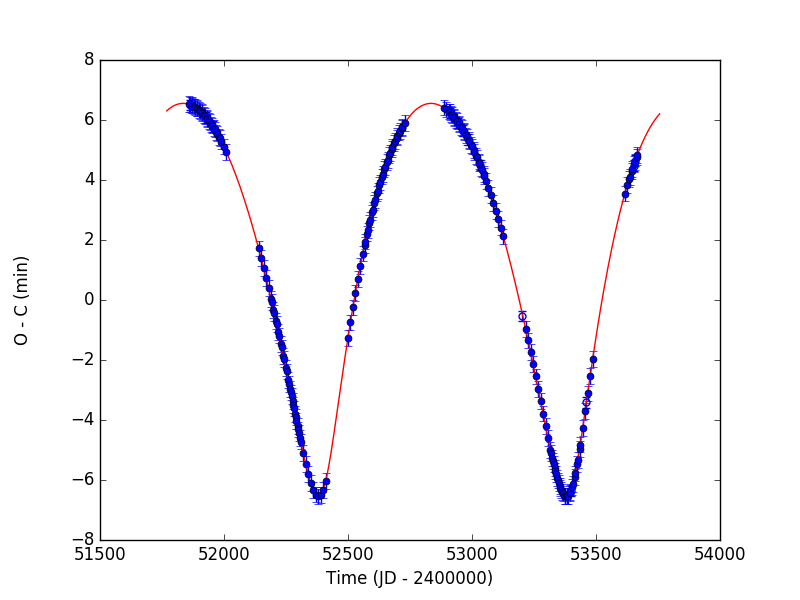
\includegraphics[width=\textwidth]{overc_ideal.png}
        \caption{o-c ideal}
    \end{subfigure}%
    \begin{subfigure}[t]{0.5\textwidth}
        \centering
        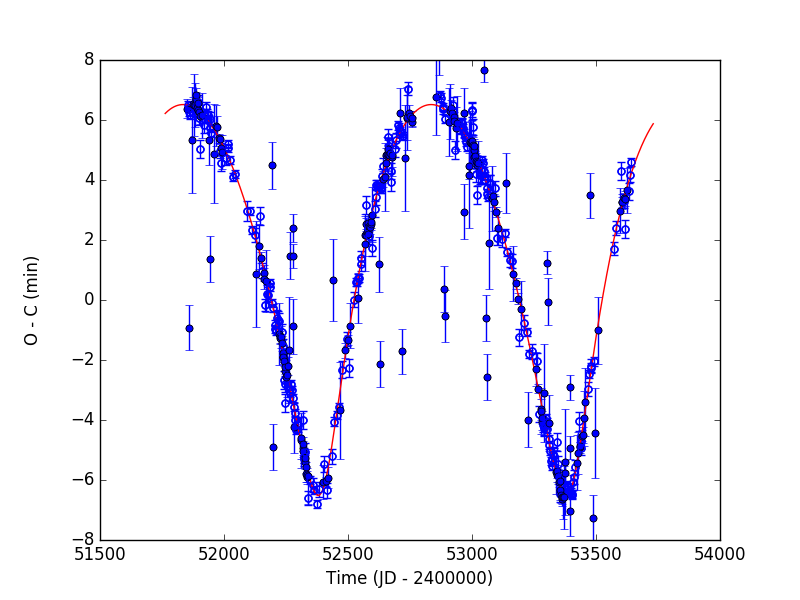
\includegraphics[width=\textwidth]{overc_spot_migr4.png}
        \caption{o-c with spot}
    \end{subfigure}
    \caption{O-C diagram for contact EB system with (b) and without (a) migrated spot.
        Red line - fit with MCMC method, correspond to values in table \ref{tab:3rd_body_overc_spot}. 
        Filled circles are primary minima, not filled circles - secondary minima.}
\label{fig:overcontact_spot_oc}
\end{figure}

From figure \ref{fig:overcontact_spot_oc} we can clearly see how migrated spot reduce precisions of minima exact time detection and in some cases, we even got point that does not fit in our O-C diagram. This means that these points are faults. Migrated spots are the most difficult cases for precise definition time of minima, make O-C diagram and define orbital parameters of $3^{rd}$ body.
Fitted parameters of orbit and $\chi^2$ values of fit are presented in table \ref{tab:3rd_body_overc_spot}. 
  
\begin{table}[!h]
 \caption{Orbital parameters of $3^{rd}$ body for contact EB system with two spots and migrated spot. Spot parameters $r_{spot}=35\degree$, $T_{spot}=0.8~T_{surf}$. For description of parameters see Table~\ref{tab:3rd_body_par}}
  \vspace{-6mm}
 \begin{center}
  \begin{tabular}{lcccc}
    \hline
    Solution            & Original       & no                  &   two        & migrated   \\
                        &                & spot                &   spots      & spot       \\
  \hline\noalign{\smallskip}                                                              
 $P$ [days]             & 1.42834        &           fixed     &   fixed      & fixed        \\ 
 $T_0$ [HJD]            & 2451852.3783   &           fixed     &   fixed      & fixed        \\
   \hline\noalign{\smallskip}                                                                                           
 $P_3$ [days]           &   1000         &          999.7(8)   &   999(1)     & 1000(1)      \\       
 $t_{03}$ [HJD]         & 2451400        &          2451400(2) &  2451402(2)  & 2451398(4)   \\
$a\sin i_3$ [AU]        &  0.797         &          0.799(3)   &  0.799(3)    & 0.764(3)     \\     
 $e_3$                  &  0.54          &          0.541(4)   &  0.532(5)    & 0.541(2)     \\            
$\omega_3$ [\degree]    &   288          &          288.1(7)   &  288.5(8)    & 287(1)       \\     
\hline\noalign{\smallskip}                                                                                         
$f(M_3)$  [M$_\odot$]   &  --            &          0.0681(8)  &  0.0683(9)   & 0.0666(7)    \\       
\hline\noalign{\smallskip}                                                                                  
$\chi^2$                &  --            &          0.614      &  6.547       & 2478.629      \\        
$\chi^2/n$              &  --            &          0.0283     &  0.0719      & 6.1200       \\       
\hline\noalign{\smallskip}  

\end{tabular}
\end{center}
\label{tab:3rd_body_overc_spot}
\vspace{-6mm}
\end{table}

\subsection{Pulsations in EB Systems}
Pulsation in eclipsing binary systems can be observed in Algol-type binaries, the so-called oEA stars (oscillating EA stars).
The oEA stars are mass-accreting main sequence A/F-type components in semidetached Algol-type eclipsing binary systems showing $\delta$~Sct - like pulsation \citep{Rodriguez2010}. The period of pulsation in such systems can vary from 20 to 300 minutes (see e.g \cite{Liakos2017}, \cite{Mkrtichian2007}). 

In work \cite{Liakos2017} relation for period of pulsation is given as:
\begin{equation}
P_{pul} = 0.031(4) + 0.009(1) P_{orb}. 
\end{equation} 

This relation is based on observation of $\delta$~Sct stars in all known close binaries systems (Detached, Semi-detached, unclassified). Coefficient of correlation for this relation is $r=0.62$.

To determine how the pulsations affect the O-C diagram and $3^{rd}$ precision of orbital elements we will consider three cases of detached EB systems with a different period of pulsations: 30, 150, 300 minutes.

To define the precise time of minima with pulsation presence it is very important to have a high rate of observation per some time interval (or per LC).
Until now we use synthetic LC generated by PHOEBE with sample rate 300 points per period. That was fully enough to precisely determine the time of the minima, but such rate is not enough for pulsations study.

To determine what sample rate should we use, let us check how the precision of primary minima is changed in detached EB system with added pulsations with parameters --- period $P_{pus}=30$ min and amplitude $A_{puls} = 0.02$. 
Three examples of same minima fitted in sample rates 300, 600 and 900 points per LC are presented on figure \ref{fig:puls_dif_rate}. If we have more than 900 points per LC then the precision of minima determination is slightly increasing to value 0.001 of a day. 
With the increase of sample rate, time of calculation also greatly increases, therefore the value of 900 points per LC is the best choice.

$3^{rd}$ body orbit parameters determined in detached EB system with pulsation with a period of 30, 150 and 300 minutes are presented in table \ref{tab:3rd_body_par_puls}. As we can see from a table, the most precise determination of orbit parameters corresponds to pulsation with the longest period. Vice versa most inaccurate parameters of orbit determination correspond to the shortest period. A short period of pulsations can't make it impossible to determine the precise time of minima, and as we show above it is also very important what resolution of LC do we have. 

\begin{figure}[!h]
    \centering
    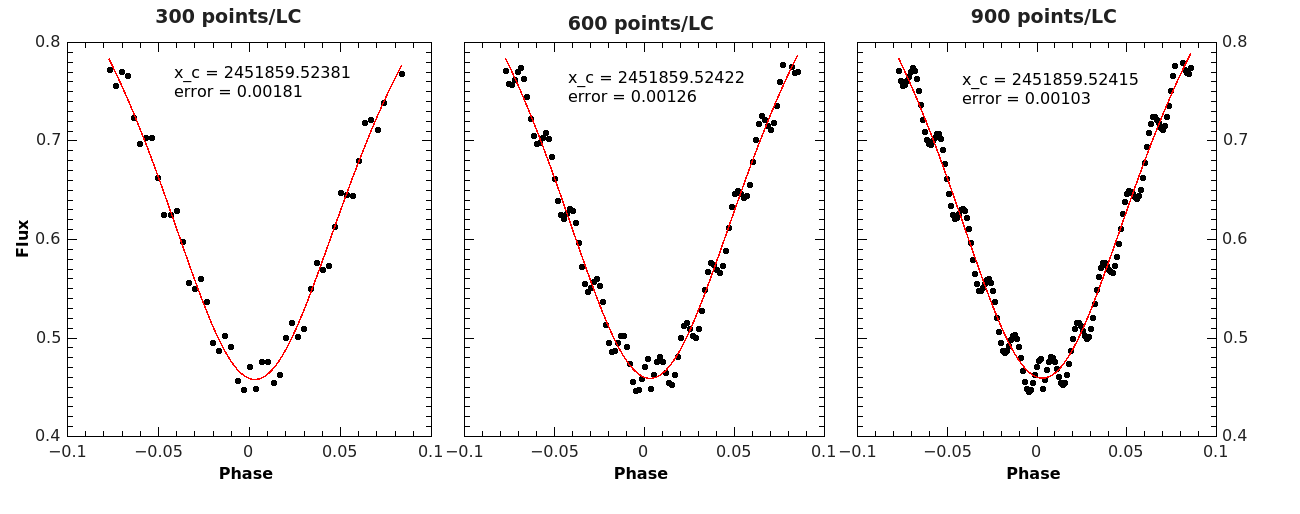
\includegraphics[width=\textwidth]{puls_dif_rate.png}
    \caption{Different sample rate and precision of primary minima determination. Black point are data from LC, red line - fitted minima.}
\label{fig:puls_dif_rate}
\end{figure}

%\begin{figure}[!h]
%    \centering
%    \begin{subfigure}[t]{0.325\textwidth}
%	    \centering
%	    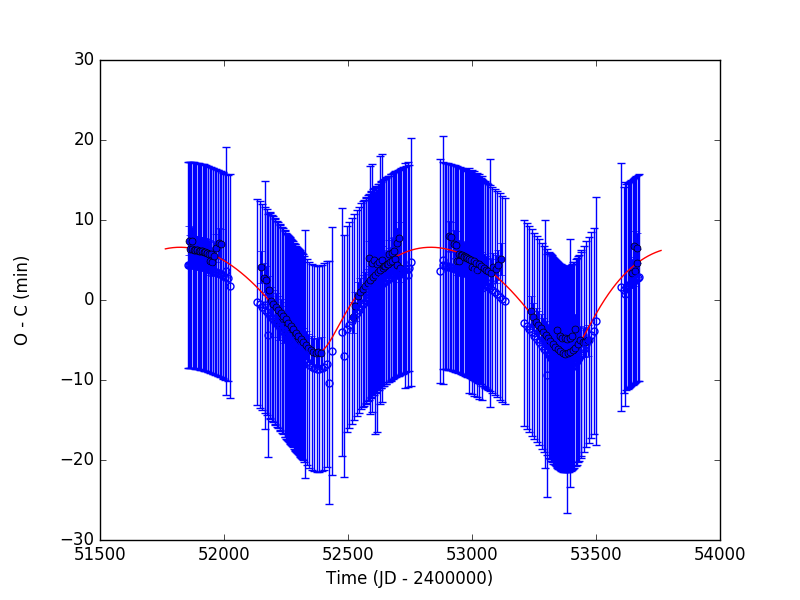
\includegraphics[width=\textwidth]{oc_puls_30m.png}
%%	    \caption{O-C diagram for 300 points/LC}
%    \end{subfigure}
%    \centering
%    \begin{subfigure}[t]{0.325\textwidth}
%	    \centering
%	    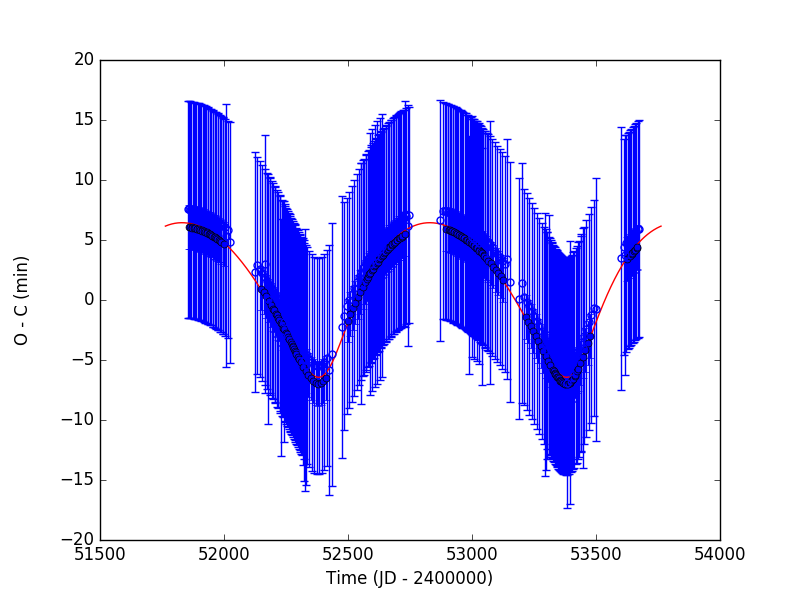
\includegraphics[width=\textwidth]{oc_puls_30m600.png}
%%	    \caption{O-C diagram for 600 points/LC}
%    \end{subfigure}
%    \centering
%    \begin{subfigure}[t]{0.325\textwidth}
%	    \centering
%	    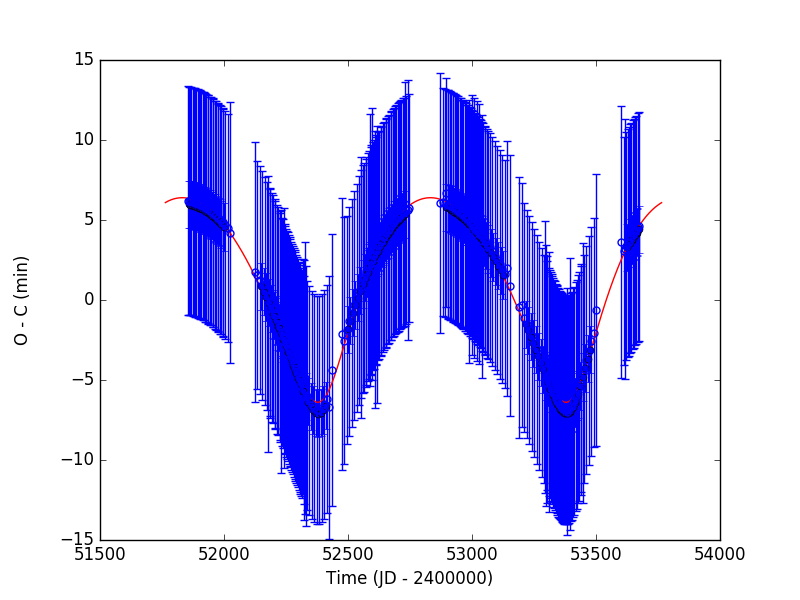
\includegraphics[width=\textwidth]{oc_puls_30m900.png}
%%	    \caption{O-C diagram for 900 points/LC}
%    \end{subfigure}
%    \caption{O-C diagrams with different sample rate. Left - O-C diagram for 300 points/LC, middle - for 600 points/LC, and right - for 900 points/LC}
%\label{fig:puls_dif_rate_oc}
%\end{figure}

\begin{table}[!h]
 \caption{Orbital parameters of $3^{rd}$ body for detached EB system with pulsations. 
 For description of parameters see Table~\ref{tab:3rd_body_par}}
  \vspace{-6mm}
 \begin{center}
  \begin{tabular}{lcccc}
    \hline
    Solution            & Original       & Pulsations         & Pulsations          & Pulsations \\
                        &                & $P_{puls}$=30 min  & $P_{puls}$=150 min  & $P_{puls}$=300 min\\
  \hline\noalign{\smallskip}                                                                                                                 
 $P$ [days]             & 1.42834        &           fixed     & fixed         & fixed        \\ 
 $T_0$ [HJD]            & 2451852.3783   &           fixed     & fixed         & fixed        \\
   \hline\noalign{\smallskip}                                                                             
 $P_3$ [days]           &   1000         &          1000(7)     & 1002(8)      &  1000(7)     \\       
 $t_{03}$ [HJD]         & 2451400        &          2451408(16) & 2451390(19)  &  2451399(19) \\
$a\sin i_3$ [AU]        &  0.797         &          0.778(19)   & 0.813(19)    &  0.807(19)   \\     
 $e_3$                  &  0.54          &          0.431(29)   & 0.600(28)    &  0.569(30)   \\            
$\omega_3$ [\degree]    &   288          &          291(5)      & 285(5)       &   288(5)     \\     
\hline\noalign{\smallskip}                                                                              
$f(M_3)$  [M$_\odot$]   &  --            &          0.0628(47)  & 0.0715(52)   &  0.0700(52)  \\       
\hline\noalign{\smallskip}                                                                          
$\chi^2$                &  --            &          8.519       & 2.778        &  0.802       \\        
$\chi^2/n$              &  --            &          0.0184      & 0.0069       &  0.0019      \\       
\hline\noalign{\smallskip}  

\end{tabular}
\end{center}
\label{tab:3rd_body_par_puls}
\vspace{-6mm}
\end{table}